% Changing book to article will make the footers match on each page,
% rather than alternate every other.
%
% Note that the article class does not have chapters.
\documentclass[letterpaper,10pt,twoside,openany]{book}

% Use babel or polyglossia to automatically redefine macros for terms
% Armor Class, Level, etc...
% Default output is in English; captions are located in lib/dndstring-captions.sty.
% If no captions exist for a language, English will be used.
%1. To load a language with babel:
%	\usepackage[<lang>]{babel}
%2. To load a language with polyglossia:
%	\usepackage{polyglossia}
%	\setdefaultlanguage{<lang>}
\usepackage[english]{babel}
%usepackage[italian]{babel}
% For further options (multilanguage documents, hypenations, language environments...)
% please refer to babel/polyglossia's documentation.

\usepackage[utf8]{inputenc}
\usepackage{hang}
\usepackage{lipsum}
\usepackage{listings}
\usepackage{hyperref}

\usepackage{dnd}

\lstset{%
  basicstyle=\ttfamily,
  language=[LaTeX]{TeX},
}

\usepackage{eso-pic}
\newcommand\BackgroundPic{%
	\put(0,0){%
		\parbox[b][\paperheight]{\paperwidth}{%
			\vfill
			\centering
			
\includegraphics[width=\paperwidth,height=\paperheight,%
			keepaspectratio]{img/paper.jpg}%
			\vfill
}}}

\newcommand\BackgroundPicAlt{%
	\put(0,0){%
		\parbox[b][\paperheight]{\paperwidth}{%
			\vfill
			\centering
			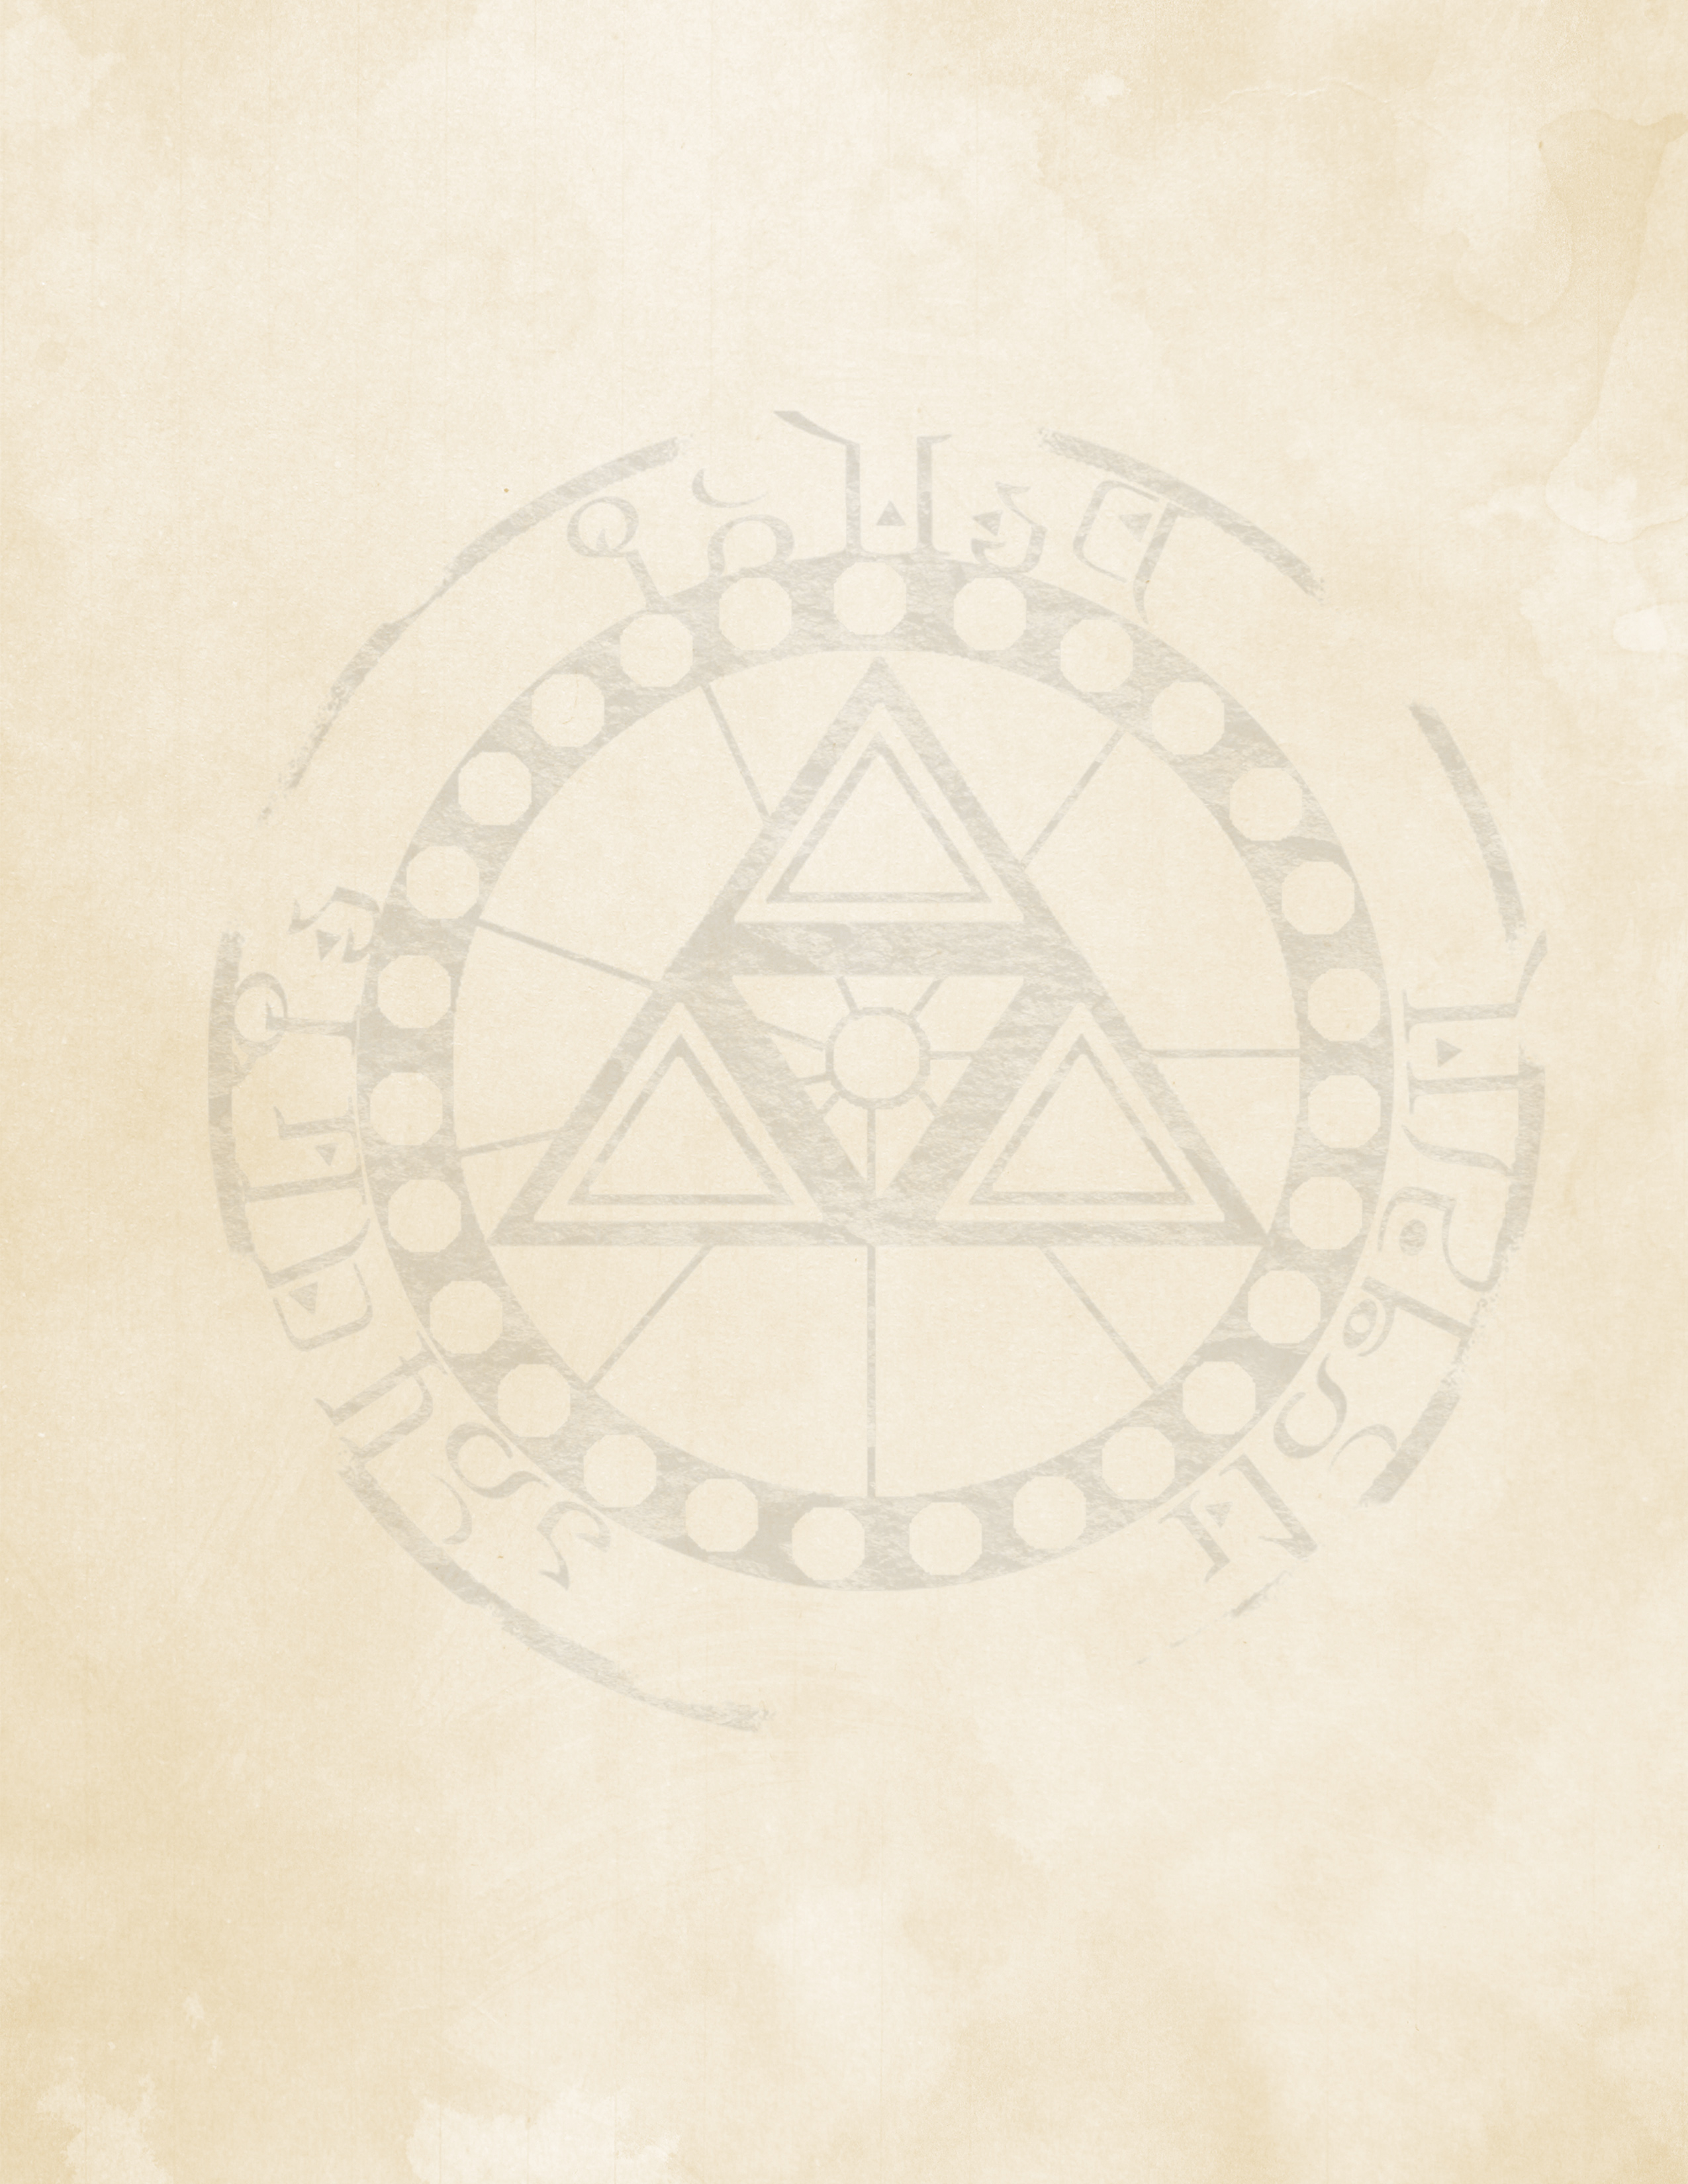
\includegraphics[width=\paperwidth,height=\paperheight,%
			keepaspectratio]{img/trinitypaper2.png}%
			\vfill
}}}

\title{The Mystery of the Trinity Stones}
\author{Antonius Torode}
\date{Latest update: \today}


% Start document
\begin{document}

\AddToShipoutPicture*{\BackgroundPicAlt}
\maketitle
\tableofcontents

\chapter{The Trinity Stones}

\section{Creation of a Trinity}

\begin{quotebox}
	In the beginning, The Celestials created the Heavens and the Earth. A singularity of reality from whence space was formed, energy was made, and time unraveled. A trinity of reality to be seen forever.
\end{quotebox}

No matter the story of beginning, it all arrives at the same principles. Space, time, and matter. A trinity of reality stemming from the creation itself. For none can exist without another, and in existence all must come simultaneously. These forces of the cosmos work in unison and cannot be broken from each other. At least that's how we've perceived it.

\section{Creation of the Stones}

\textbf{It is said} that those who can harness the power of reality itself would have unrivaled power. The outcomes of reality itself would be for them to decide. Unfortunately to harness the trinity would be to harness the universe, a space incomprehensible to perceive. In ancient times, there existed an organization known as the Celestial Guard. This group of people extended through all races and across the entire world. A common goal among them was to understand and tap into this trinity. Through centuries, hidden mysteries of the universe began to be unraveled, bringing forth the secrets of magic and powers known today. The Celestial Guard was the primary source of the advancements of knowledge. It is said that the knowledge and understandings of these ancients vastly surpassed anyone from todays era. 

Over time, the Celestial Guard became segregated. After discoveries pertaining to parallel realms, there became hidden agendas. A civil war on a global scale ensued among the Celestial Guard. A war on such great of a scale that the majority of knowledge was lost as a consequence. As it is told, the council of seven (the last leaders of the Celestial Guard) had unlocked an understanding that has never before been known. Through this they were able to create what we call the Infinity Stones. 

A minuscule part of reality was harnessed into three stones, space, time, and matter. Each stone is unique in appearance but all mesmerizing in appearance. The stones are said to bring immeasurable powers to the users. Not by their powers themselves, but through the understanding they bring. The stones were created as a milestone in understanding. Unfortunately, due to the war and the hastily actions of the council, the stones were hidden away. A powerful spell was placed on the stones such that they cannot be found save all together. If any stone is found apart from a counterpart, reality itself will bend around the stone, hence placing it back in hiding. 

The stones have a unique ability to act on their own each in a unique way. Each stone has a unique look which three sections. The stones are cut in such a way that they all fit together. The stones each have remnants of the others glow within it and parts of each stone will turn dark when the others are not near. 

\section{The Celestial Guard}

The legend of the Celestial Guard is an ancient world-wide coalition of beings. The Guard was started by a group of elite warriors whom banded together to dethrone a corrupt kingdom. Seven warriors in total were among the original Guard. They were able to take down an entire kingdom from within and established a new council of seven where their goals and actions carried enough wait to gain the allegiance of the masses. After establishing a new government, they created what was known as the Celestial Guard, where knowledge and understandings were all but the property of the world. 

Once established, the advancements of the era accelerated at a growing rate. This was before the time of wizards and sorcerers. However, through time, as secrets became unraveled, these classes became commonplace. Each generation, the council kept the same size of seven. Seven elite members based on their accomplishments. After a few hundred years, the council became involved with the discovery of the trinity of reality. The focus of the council's research became focused on this and this alone. Breakthroughs in this field lead to new spell discoveries and new ways to shape reality. Unfortunately the surface of knowledge was barely scratched, until one day.

In one era, a generation of six master sorcerers, wizards, and warlocks existed as part of the council. The seventh member was a warrior named Kurdran. It was rare that the whole council would get together, and just as rare for only six of them to get together. There was a find by one of the members, however, where all of the members got together save Kurdran. Together, the six members explored a new concept that one of them had discovered. After only a few short days, a rift in space was created. A single point in space was expanded and shown to contain energy and time in the absence of space (at least, the space that had been known about). This was the void. The six members were not prepared for what followed and one of them was lost to sealing the rift. This rift had unforeseen consequences throughout all of space. Space became unstable and rifts began to appear at random.

This incident created changes on a global scale, which negatively impacted the incentives of many. New possibilities in magic were being opened to many. The council was now down to six total. Somehow, through a chain of small events, news got out of the council and rumors were put together with the new changes that the rift brought. The council was blamed and civil war broke out. This was a war to drown out all other wars. The war went on for years, between new factions that had broken out within the Celestial guard. The six council members appeared to have all dissipated. In reality, they were hidden. With the opening of the void, plane shifting was now an option. The council members banded together as six hidden in reality on a new plane. There they were able to focus on their studies. They believed the only way to reverse what they had done with the initial rift is to understand the other elements of the trinity. 

First, the council had to disrupt time itself, creating a reality of only space and matter. One mistake doing this and they would have been trapped in a single moment for eternity. Following this, matter had to be torn from reality to 
create existence pertaining of only space and time. A pure vacuum in which anything matter would be instantly annihilated. With each advancement, reality itself became more unstable. It took much time, but after learning what they could about these new realities, they knew how to stop the chaos. This is when the Trinity Stones were created. The stones were containers for the tears in our reality. They each bear the power of the trinity to seal each individual tear in reality.

Among returning from hiding, the world was shattered. While away, the void realm had consumed many, time had been warped, energy expanded out of balance. The trinity stones ended the chaos, but the damage was irreparable. The Celestial Guard was no longer a thing, for the members had all been scattered, destroyed, or changed. The stones were then sealed away, behind a powerful spell. The last act of the council before they disbanded. The members each went their own way in order aid and rebuild in different locations. Over time, the Celestial Guard was forgotten by most. The world grew into a new place as it is today and all of this only exists in mere legend.  

\section{The Space Stone}

The space stone controls elements pertaining to spacial events. The space stone mainly causes objects to randomly move location.


\section{The Matter Stone}

The matter stone controls elements pertaining to power and lack thereof. The matter stone primarily causes illusionary events such as glowing ponds and rivers as well as transforms beasts into both stronger or weaker than they usually would be.

\section{The Time Stone}

The time stone controls temporal events. The stone primarily will cause objects to teleport into different locations within the flow of time.

\section{The Celestials}

The reality of the Myths laid by the Trinity Stones follow from an Ancient sect developed from the Celestial Guard. The understandings brought about by the age of the celestial guard lead to greater understandings of consciousness\footnote{The Ideas for this are from Stargate SG-01} and the infinite universe. The world was not thrown into chaos like legend claims but rather destroyed by its own inhabitants a millennium later. Within a few thousand years of research and after the creation of the stones and understandings brought about from the multidimensional discoveries of the time, a sect of beings discovered a way of shedding their spirits from their physical bodies and existing on a higher plane of existence. 

This shedding of the soul was known as ascension and was seen by many as a way of ultimate understanding. Unfortunately some of these beings discovered there was a connection between the mortal souls and the ascended souls and in the mortals worshiped the ascended beings their power and understanding was enhanced. Others decided that with this existence as an ascended being, they do not have the right or purpose or need to affiliate with lower life forms and took off into the universe to gain a greater understanding. The ascended beings who stayed called themselves the celestials after the Celestial Guard and believed they had achieved the ultimate destiny and form of understanding. These beings looked at themselves as gods and thought it appropriate to rule over the lower beings.

The Celestials created a religion known as Celestus in which they had mortals worshipping them with the false hope of ascension. The religion was based on the Celestus Writings (or the Book of Celestus). Through time, the celestials convinced all of their followers that the unbelievers must be destroyed which inevitably lead to world wars. This lead to the destruction of almost the entire population and loss of most knowledge. The myth of the Trinity stones was preserved through a group of knights lead by Myrddin who was a member of a breakoff group from the Celestial Guard known as the Alterans. 

Through the power of the Celestials, they "enhance" individuals (priors of Celestus) to spread the word of Celestus throughout the lands. These priors cannot easily be defeated because they have powers pertaining to understandings from the Celestials that protect them. However, the priors are generally peaceful and only harm via the armies they command. They will send themselves in if something really needs done but mainly stick to preaching while their armies are off conquering. After the destruction of the world, many centuries went by as the Celestus followers rebuilt their population as well as the rest of the planet did too.

\section{Myrddin}

Myrddin was an Alteran. His name, Myrddin can also be translated to Merlin, regarding Merlin and the knights of the round table. Merlin was a member of the Celestial guard whom figured out the secrets to ascension but saw the negative consequences it could have on the planet and universe. He decided to not ascend himself and instead rebelled against the Celestials. In doing so, none of the other Alterans (the ones who could ascend) stayed with Merlin and he was left alone with his beliefs. Myrddin was one of the first to determine the secrets behind ascension and was one of the most knowledgeable of people at that time.

Myrddin put it upon himself to create a technology allowing him to destroy ascended beings, which was not thought possible. However, he could not do such a thing outright because the Alterans and Celestials would have interfered and destroyed him, but instead he had to find a way to mask his work by shifting himself between dimensions. He was able to create a device known as the San'graal (The Holy Grail) which had the capabilities of destroying the Celestials but was unable to activate it due to him closely being watched by the Celestials. Myrddin instead left his work hidden behind secrets, like the Trinity stones and kept his secrets safe guarded by the knights of the round table throughout the generations.

Myrddin's end research was left in a secret lab which can only be accessed via the Trinity stones. Myrddin froze himself in stasis within his lab and he contains the knowledge of how to create the San'graal by it's base particles. If the Trinity Stones are fitted together (after being found of course), the users will be transported to Myrddin's Laboratory. Myrddin and his various other labs were all location in the Pluvian Forest. One of such places is referred to as Avalon which is a place where him and his knights kept all of the treasures from that age.

\section{Morgana}

Morgana (also known as Morgen Lafe) was an Alteran from Myrddin's time. She was greatly opposed to Myrddin advancing his capabilities to combat ascended beings due to her plans to ascend herself. Unfortunately, due to herself convincing that Myrddin succeeded in creating the San'graal, she never ascended herself. She dedicated her life to studying the Trinity stones and to determine Myrddin's secrets to destroy the San'graal before ascending. However, during her lifetimes, she was able to understand the true threat that the Celestials posed and changed her mind to side with Myrddin. Myrddin was significantly more clever than Morgana and Morgana determined that there were safeguards around the San'graal preventing her from finding it. Due to this, she is lying in wait to assist those who can actually find it. 

 



\chapter{The Campaign}

\subsection{Tempestas}

At the start of the campaign, the DM needs to decide on a reason for the characters to be coming into Tempestas. This can be any good reason that fits with the player backstories or one from the following list. Tempestas is a large city with many things to do. The city will start closed off due to the impending threat of the Celestials attacking nearby cities. From Tempestas, the players can be lead to Aurushire. Different reasons can lead them to Aurushire such as the sport of the jungles or the search for the Trinity stones. Little do they know that the Trinity stones are the key to obtaining the San'graal to defeat the Celestials.

The players can start out in Tempestas either by living there, being in the prison there, or arriving there by spice trade (depending on the character backgrounds). While in Tempestas, they can encounter a few important characters such as Dastan and the fortuneteller. While in Tempestas, a Prior of the Celestas will also arrive and start his preaching. 

\subsection{Journey to Aurushire}

\begin{commentbox}{Journey to Aurushire}
	\begin{description}
		\item[For the Stones] Legend has it that there are rare and priceless artifacts hidden on Statu. It is possible that the player could be hunting the legends which have lead them to Aurushire.
		\item[The Rare Sport of Rem Silva] It is possible that the rare game in Rem Silva was spoken of and the players could be after the rare sport that resides in this area.
	\end{description}
\end{commentbox}

After leaving Tempestas by boat (If the party gets to this), they will have some rest time on the ship they are on. The tripe is generally only about a day or two away from Statu, however the party will encounter rough weather. The rough weather will turn into a massive storm in which the ship will be knocked around, back and forth. The party will be knocked unconscious and awake on the coast due east on Aurushire (without knowing of course) with only the players that are in their party and none of the NPCs from the ship. The cost will have rock and cliff faces to their east, and rough forest and mountains (appears unclimbable) to the North. Their only option is the the west. The west will lead into the Convallis swamp and marsh area's which is directly east of the Naga encampments. A thick fog will appear as they are traveling and they will need to navigate through rough swampy regions where they will encounter serpent Naga forces and some magical beasts like a witch hunter. After navigating through this region, the party will arrive and Aurushire, battered and beaten.

After arriving at Aurushire, there are many options for the players. There is an Inn (Prancing Pony Inn), where they can get rest. There are farms, where the players could potentially work. There are the mines, run by a Pandaren brother, where players could also work. There is a blacksmith, which is run by one of the three Pandaren brothers. There is the brewery/tavern, which is run by another Pandaren brother for players to socialize, learn, and relax. There is also Bob's Guns. Bob is a strange fella who claims is he from a more modern time. He has things that you cannot find anywhere else. To the northeast there is an old witch named Yaga. To the northwest a wizard named Baba. Together the two are sometimes referred to as the Ying-Yang. For one appears good, and one appears the opposite. Though this name comes from the matter of looks, and not actions. 

\subsection{Baba}

Baba is a powerful wizard who has spent many lifetimes studying the flow of time and impacts of the time stone on the surrounding regions. Baba can be found throughout the time line as different versions of herself. At one point she found a way to manipulate the temporal and spacial fluctuations throughout the region to create copies of herself in different space-times. From this, there are Baba's hidden throughout the time line all living as separate entities. 

Baba's role can be whatever the DM likes. She was intended to persuade the users to seek the trinity stones. Along with this, Baba knows the powers and trickery of the stones and would not believe the party is ready no matter how experienced. Because of this, she can teleport them to various locations for trials such as the halls of no end \ref{maps} or the various surrounding regions. 

\begin{center}
	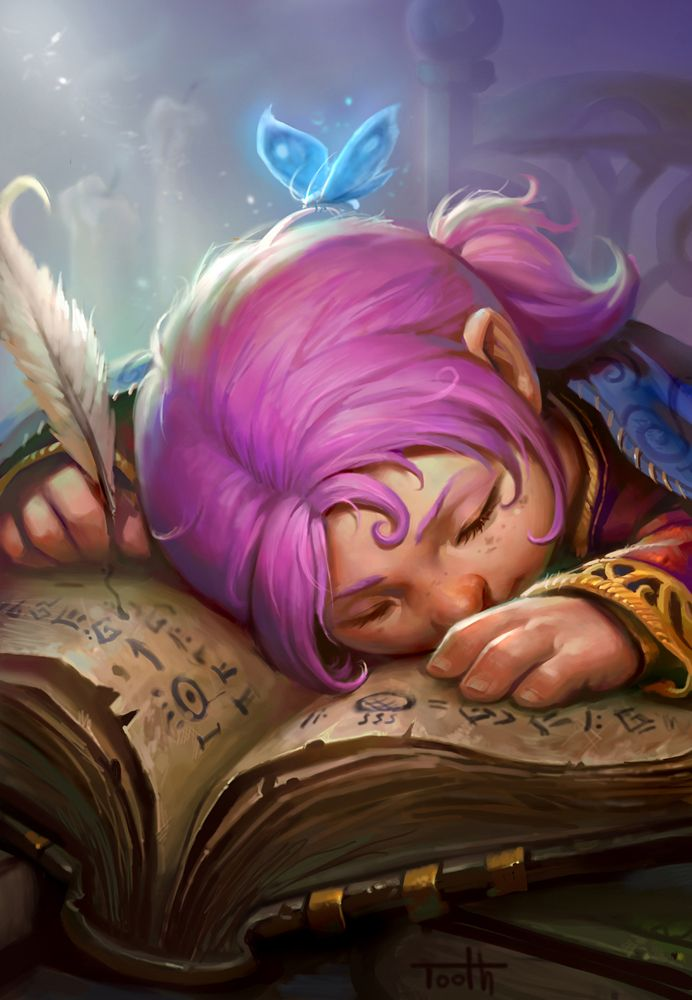
\includegraphics[width=0.5\linewidth]{img/baba.jpg}
\end{center}

\begin{monsterbox}{Baba}
	\begin{hangingpar}
		\textit{Gnome Wizard, Neutral Good}
	\end{hangingpar}
	\dndline%
	\basics[%
	armorclass = 24,
	hitpoints  = 302,
	speed      = 60 ft
	]
	\dndline%
	\stats[
	STR = \stat{8}, % This stat command will autocomplete the modifier for you
	DEX = \stat{16},
	CON = \stat{19},
	INT = \stat{20},
	WIS = \stat{20},
	CHA = \stat{19}
	]
	\dndline%
	\details[%
	% If you want to use commas in these sections, enclose the
	% description in braces.
	% I'm so sorry.
	languages = {Common, Elvish, Dwarvish, Gnomish, Halfling, Orc, Pandaren, Celestial, Draconic, Primordial},
	challenge = 20
	]
	\dndline%
	\begin{monsteraction}[Telekinesis]
		The ability to move objects with your mind. There is no limitation to how the objects can be moved if the objects belong to you.
	\end{monsteraction}	
	\begin{monsteraction}[Cerebral Warp]
		You can place humanoids into a deep illusion that seems completely real. The subjects cannot be harmed in the illusion.
	\end{monsteraction}	
	\begin{monsteraction}[Illusionary Presence]
		When you are near others, you feel to them to be in multiple places at once. If struck by a melee attack, you can relocate to an alternate location within 10 feet.
	\end{monsteraction}
	\begin{monsteraction}[Precision Striking]
		When you attack, you can choose hwo much damage to deal up to the amount shown on the attack roll.
	\end{monsteraction}
	\monstersection{Actions}
	\begin{monsteraction}[Spells]
		A lot of spells.
	\end{monsteraction}
	\monstersection{Description/Information}
	Baba lives in seclusion. She is an extremely small gnome that does not mind helping others when asked. She is extremely intelligent and powerful, even though she does not look it. Baba is very old, however, very well kept and appears young.
\end{monsterbox}

\begin{commentbox}{Baba's Wizard Hat}
	Baba's hat has a mind of it's own. As a good way to show the personality of Baba, the Hat she wears can move on it's own, showing emotion and performing magical acts. As an example, if someone says something surprising to Baba, the hat itself can do a sort of 'eyebrow raise'. Also, when Baba walks forward, the hat could remain stationary and come off of her head if it's surprised or distracted. The hat is similar to the hat from Harry Potter only it cannot speak and does not have a mouth or eyes.
\end{commentbox}

\begin{commentbox}{Baba as Morgana}
	Within the campaign, Baba can be used as Morgana. Myrddin was much more crafty, intelligent, and clever than Morgana was. In regards to creating the San'graal, he created the Trinity stones and was able to manipulate and parse through temporal (time) events. Due to this, he was able to hide his clues throughout time. 
	
	Morgana realized this but did not have the same understanding and Myrddin. She found a way to manipulate the trinity stones in order to essentially clone herself throughout different space-times. This has allowed Baba to wait in different temporal locations for mysteries of Myrddin.
\end{commentbox}

\begin{commentbox}{Baba as Morgana's sister}
	Within the campaign, Baba can be used as Morgana's sister. Myrddin was much more crafty, intelligent, and clever than Morgana was. In regards to creating the San'graal, he created the Trinity stones and was able to manipulate and parse through temporal (time) events. Due to this, he was able to hide his clues throughout time. 
	
	Morgana realized this but did not have the same understanding and Myrddin. Her sister, Baba found a way to manipulate the trinity stones in order to essentially clone herself throughout different space-times. This has allowed Baba to wait in different temporal locations for mysteries of Myrddin. After thinking her sister was a bit crazy for all of the things she spouted off about Myrddin, later in her life she discovered anomalies that supported the things her sister claimed. She eventually turned towards studying the mysteries left by Myrddin.
\end{commentbox}

\begin{commentbox}{Baba's Tower}
	Baba resides in a mage tower that lies about a day's journey to the northwest of Aurushire. The tower is multileveled and has a winding wooden staircase that leads all the way to the top level of the tower. The tower contains many different books and brewing stations among it's level. The tower has a hollow center where the top can be seen from the bottom. The top level is larger than all of the other but other than that level, the tower slightly narrows from bottom to top. At the top level, Baba has a view of a large portion of the surrounding regions ans it reaches just above the tree line. One thing the party may try to do is look for books throughout the place. Baba has lifetimes she has been studying and can speak many languages. Because of this, she has books of all sorts of languages. On the first level of the tower is living area's, with couches, a fireplace, tables, chairs and a very cozy and comfortable looking arrangement. As the levels go up, there are different forms of information leading to the top level where Baba has all of the high level information that she needs quick access to for studying.
\end{commentbox}

\begin{commentbox}{Kharazan}
	Kharazan is a tower that is about a 3 days journey to the northeast of Aurushire. Kharazan is a huge but semi-deserted castle. The place is old and many parts of it are broken down. There are many rooms in it such as a ballroom, full storehouse, large dining halls, dungeons, libraries, theaters, etc (Modeled similarly to the Kharazan castle in World of Warcraft). This place is where Yaga resides deep into one of the libraries of the castle up in one of the highest castles. Most of the things found within the castle are dust covered and appear to have not been used in many years.
	
	At the entrance of the castle lies a sleeping curator. This is a robotic like creature (very large) that will awaken if anyone enters the place. This curator is not hostile unless provoked or protecting the castle. This curator serves the master of the castle and can be used to give information or lead the party to where they need to go. Throughout the castle, there is a faint tune playing continually that is caused by an enchantress' spell created after the castle was abandoned.
\end{commentbox}

\begin{center}
	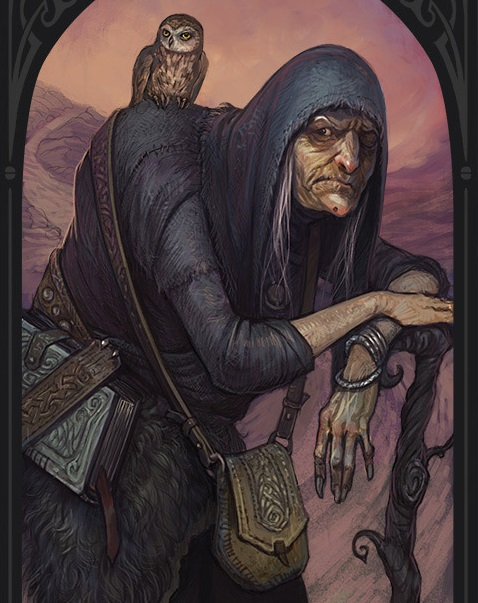
\includegraphics[width=0.5\linewidth]{img/Yaga.jpg}
\end{center}

\begin{monsterbox}{Yaga}
	\begin{hangingpar}
		\textit{?? ??, Neutral ??}
	\end{hangingpar}
	\dndline%
	\basics[%
	armorclass = ??,
	hitpoints  = ??,
	speed      = ?? ft
	]
	\dndline%
	\stats[
	STR = \stat{}, % This stat command will autocomplete the modifier for you
	DEX = \stat{},
	CON = \stat{},
	INT = \stat{},
	WIS = \stat{},
	CHA = \stat{}
	]
	\dndline%
	\details[%
	% If you want to use commas in these sections, enclose the
	% description in braces.
	% I'm so sorry.
	languages = {Common},
	challenge = 20
	]
	\dndline%
	\monstersection{Description/Information}
	Yaga is an old sorcerer. Not much is known about her. She is tall and frail (or at least appears so). It is impossible to tell anything about her from looking at her. This NPC is a wild card. It can be used with the story as seen fit (save the important things she contains to the campaign).
\end{monsterbox}

\begin{commentbox}{The Ying-Yang}
	The Ying-Yang (Baba and Yaga) plays an important part of this campaign. 
	
	Baba is a wizard that is interested in helping the party learn. She contains a vast library of knowledge and knows much about the Trinity stone legends and myths. She can assist the party in learning more. Similarly, she will insist the party is not ready if they claim they are seeking Athereu and if they insist they are will put the party through tests to confirm it. One test is to teleport the party to the halls of no end. Another would be to send them into Rem Silva after something that would help them on their journey. These challenges would be designed to assist them in their journey. 
	
	Yaga is an old witch. She appears to contain vast knowledge of the trinity stone legends as well, but acts as if she knows nothing. She can assist the party in acquiring clues and items that will help find their way to their goal. Specifically, she contains a map of Aethereu (the inside) which appears as a blank piece of paper until entering Aethereu. This map is pivotal to easily navigating the chamber. Alternatively, she can contain clues regarding successful passage through The Pluvian Forest, along with Baba.
\end{commentbox}



\begin{commentbox}{Samilah}
	Samilah, which is a name derived from Samson and Delilah meaning ``shining night''. She can be placed into the campaign in many ways but serves as the mortal embodiment of the Celestials. Her main goal is to destroy the San'graal which is the only mortal weapon known to be able to destroy the Celestials. She can disguise herself as any other sentient being and has a necklace that will protect her from any harm. She is mentally disciplined so that her mind cannot be messed with and has nearly unlimited capabilities. After destroying the San'graal she will lead the Celestial army in the conquest of Orilla.
	\begin{center}
		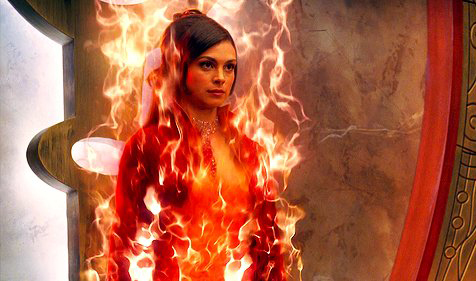
\includegraphics[width=0.7\linewidth]{img/samilah.jpg}
	\end{center}
\end{commentbox}

\begin{commentbox}{Gravemind}	
	The Gravemind is a creature modeled after the Gravemind from the Halo series. It's appearance and voice mirror that of the Halo creature but it's purpose is expanded for use in this campaign. This creature has existed since before humanity. It lives deep in the Earth and prefers warm and humid climates. The creature is not very mobile as far as relocating its self, however it is extremely agile in battles as it has a large amount of tendrils that can poison, paralyze, attack and more to anything it desires. The creature typically travels through a cave system that exists on volcanic fault lines under oceans. 
	
	Where the creature can appear in the campaign can vary but is typically if a player, or the party finds themselves adrift in the ocean or body of water. The creature needs a large amount of time to surface and show itself. It can also extend its tendrils vast distances and could collect objects or people from long distances away (such as under a body of water). It does need a large amount of time to do this so the target would need to be immobilized or inanimate. The gravemind is well aware of most things occuring on the surface of the planet as it can hear through rock and metal and continually watches and learns as the species of the planet develop. The Gravemind has rarely been seen throughout history but some Legends and stories have arose from it such as that of the Loch'Ness Monster and that of a flood invasion.
	
	\begin{center}
		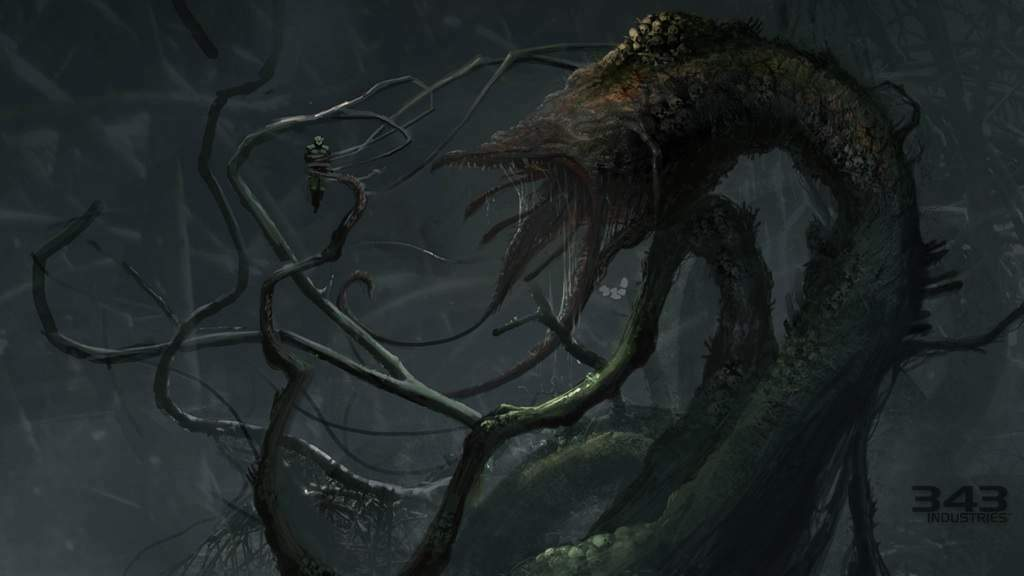
\includegraphics[width=0.6\linewidth]{img/gravemind.jpg}
	\end{center}
\end{commentbox}

\begin{commentbox}{Neokoros}
	The gravemind can lay an offspring by intertwining a bit of its DNA into another creatures nervous system. The offspring is known as Neokoros and grows in strength as the player grows. This offspring can act on it's own and becomes part of its host (similar to Venom from the spider-man series). As time passes, it can develop a relationship with the host or overtake them. Instead of having it's own turn order and stats, it instead increases the stats of a player when active. The creature can activate when it desires. If the player has a relationship with the creature, it can have some influence on when the creatures abilities activate. The main purpose of the creature is to do whatever the Gravemind gave it as its mission. For the purposes of this campaign, it's mission is to find the Trinity Stones and destroy the Celestials, though it doesn't know this precisely until the creature grows and develops more. The consciousness of the creature will slowly unravel over time.
	
	The appearance of the Neokoros can vary greatly. One method of such appearance is to appear as an alien eye within the host. The eye would have small purple veins that were not there before the infection that stem from the eye on the side of the hosts head. The parasite cannot be removed without killing the host player. Abilities of the Neokoros are determined by the level of the host creature.
	
	\begin{description}
		\item[Level 1:] The creature can telepathically communicate with the player, occasionally speaking single words or phrases.
		\item[Level 2:] The creature can sometimes move the host when the host is unconscious.
		\item[Level 3:] The creature can sometimes provide a strength success when the host is acting with their reflexes. 
		\item[Level 4:] The creature can sometimes provide an increase in combat abilities of the player.
		\item[Level 5:] The creature begins to communicate more with the host alerting the host that it has a conscious.
		\item[Level 5:] The creature can sometimes control the player while the player is conscious.
		\item[Level 6:] The creature can create visual hallucinations for the player.
		\item[Level 7:] The creature will try to either manipulate or befriend the host.
		\item[Level 8:] The creature provides a permanent +1 to strength to the host as it begins to alter the host internal cellular structure.
		\item[Level 9:] 
 	\end{description}
\end{commentbox}


\chapter{The Zones}
	
\section{Orilla}

The planet the campaign takes place on is known as Orilla. Orilla is vastly larger than Earth. It is made of large continents that span a huge ocean. The area of land mass is about six times that of Earth. For this reason, there is a large separation between different regions. Orilla is rich in neutronium which plays a pivotal role in the technological advancements of the time of the Celestials. The climate of Orilla varies based on location. The southern regions are colder but most area's are tropical and mountainous. There are some desert regions in the north east.

The majority of the planet is water. There are many volcanic fault lines all throughout the ocean which form a tunnel system under the mantel. There are volcanoes all around the planet as the size and make-up of the planet causes the inside to be greatly unstable. Storms on the planet can be much more significant and intense than those that would be found on Earth due to its size. The wind is generally calm but storms can last significantly longer and sometimes months. Due to the large variety and length storms can have, this makes travel between islands and larger regions difficult.

Orilla is largely composed of large islands (roughly the scale of Alaska). There is a southern ice region but a warm northern region. There is one large continent with a huge sea in the middle of it.

\begin{center}
	\includegraphics[width=\linewidth]{img/maps/Orilla.jpg}
	
	{\textbf{Orilla:} The massive planet of Orilla}
\end{center}

\begin{center}
	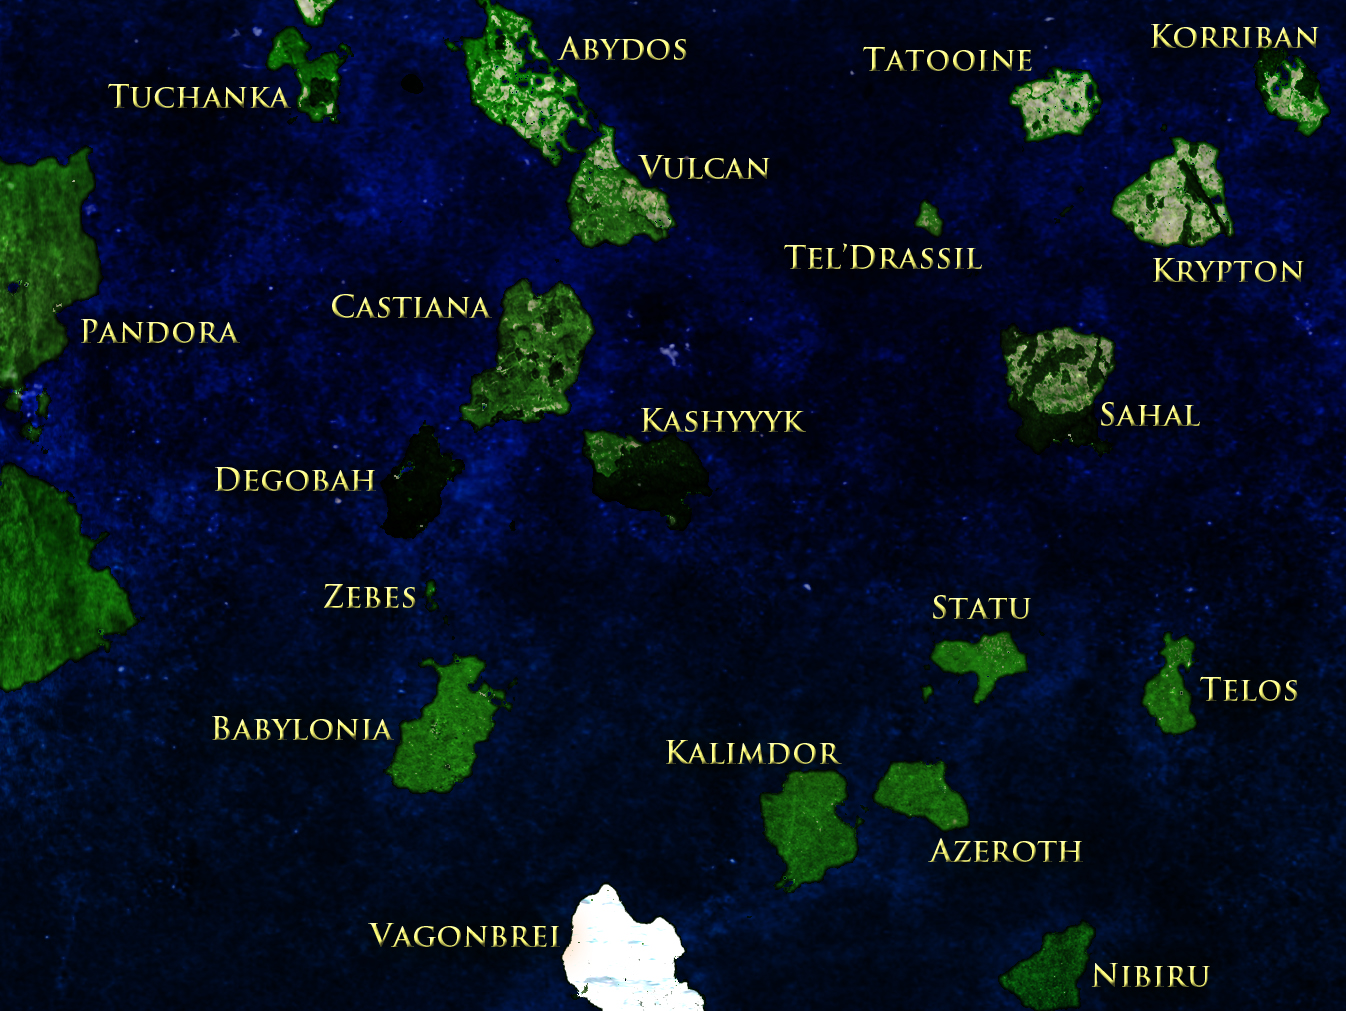
\includegraphics[width=0.7\linewidth]{img/maps/Orilla_SE.jpg}
	
	{The south eastern region of Orilla.}
\end{center}

\subsection{Regions}

The various regions of Orilla are all surrounded by water which gives them (in most cases) fertile land that is good for development of civilization. The regions are generally very large and each unique in many ways.

\subsubsection{Azeroth}

Azeroth is the home of the humans. It appears over time, the humans mainly settled in this region though they can be found in other areas. The most well known cities of this region are Tempestas which is a vast trading city that has sea ports leading to many other regions. 

\subsubsection{Degobah}

This region is similar to the Degobah planet found in Star Wars. It is largely swamp, marsh, and forest with few large mountains. The terrain is relatively smooth as far as elevation but with small hills throughout the entire region. There are many creatures here that cannot be found anywhere else on Orilla. Most of the creatures here are use to warm humid places. 

\subsubsection{Kalimdor}



\subsubsection{Tel'Drassil}

Tel'Drassil is the home of the night elves. The island is extremely dense with forest and nature and contains a unique lush type of Asheville trees that do not grown in any other region on Orilla.

\subsubsection{Abydos}

\subsubsection{Vulcan}

\subsubsection{Tatooine}

This region is largely desert. This is one of the driest regions in Orilla with almost zero humidity in some areas.

\subsubsection{Korriban}

Korriban is mostly dessert and burried history. The region is extremely windy and mountainous. There is little vegetation due to the regions past. The region contains many old temples and ruins from ancient times. There are also pyramids and large skeletal corpses scattered throughout the land. 

\subsubsection{Krypton}

\subsubsection{Sahal}

\subsubsection{Tuchanka}

\subsubsection{Pandora}

This is the largest land mass on Orilla.

\subsubsection{Babylonia}

\subsubsection{Vagonbrei}

\subsubsection{Statu}

Statu is one of the most underpopulated lush region on all of Orilla. The entire island is largely surrounded by sheer mountainous cliffs which make it difficult to travel deep into. 

\subsubsection{Telos}

\subsubsection{Nibiru}

\subsubsection{Kashyyyk}

This area is a mix of mountainous region, beaches and mountains. The jungle regions of Kashyyyk are some of the denses in all of Orilla.

\subsubsection{Castiana}

\subsubsection{Zebes}

	
	
\section{Tempestas}

Tempestas is a large city located in the south west region of the world. This is a major trading location for people all over the region. A map of the different things found in Tempestas can be seen below.

\begin{center}
	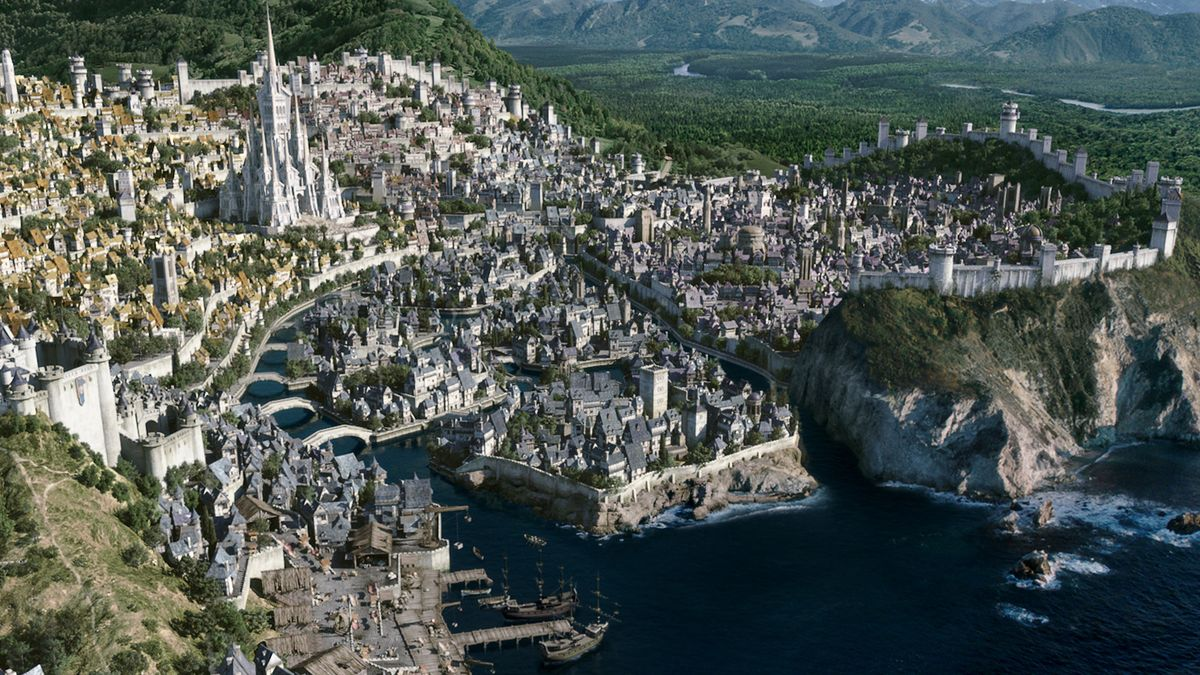
\includegraphics[width=\linewidth]{img/1200px-StormwindPanorama.jpg}
	
	{Tempestas: Tempestas is a marvelous sight.}
\end{center}

\begin{center}
	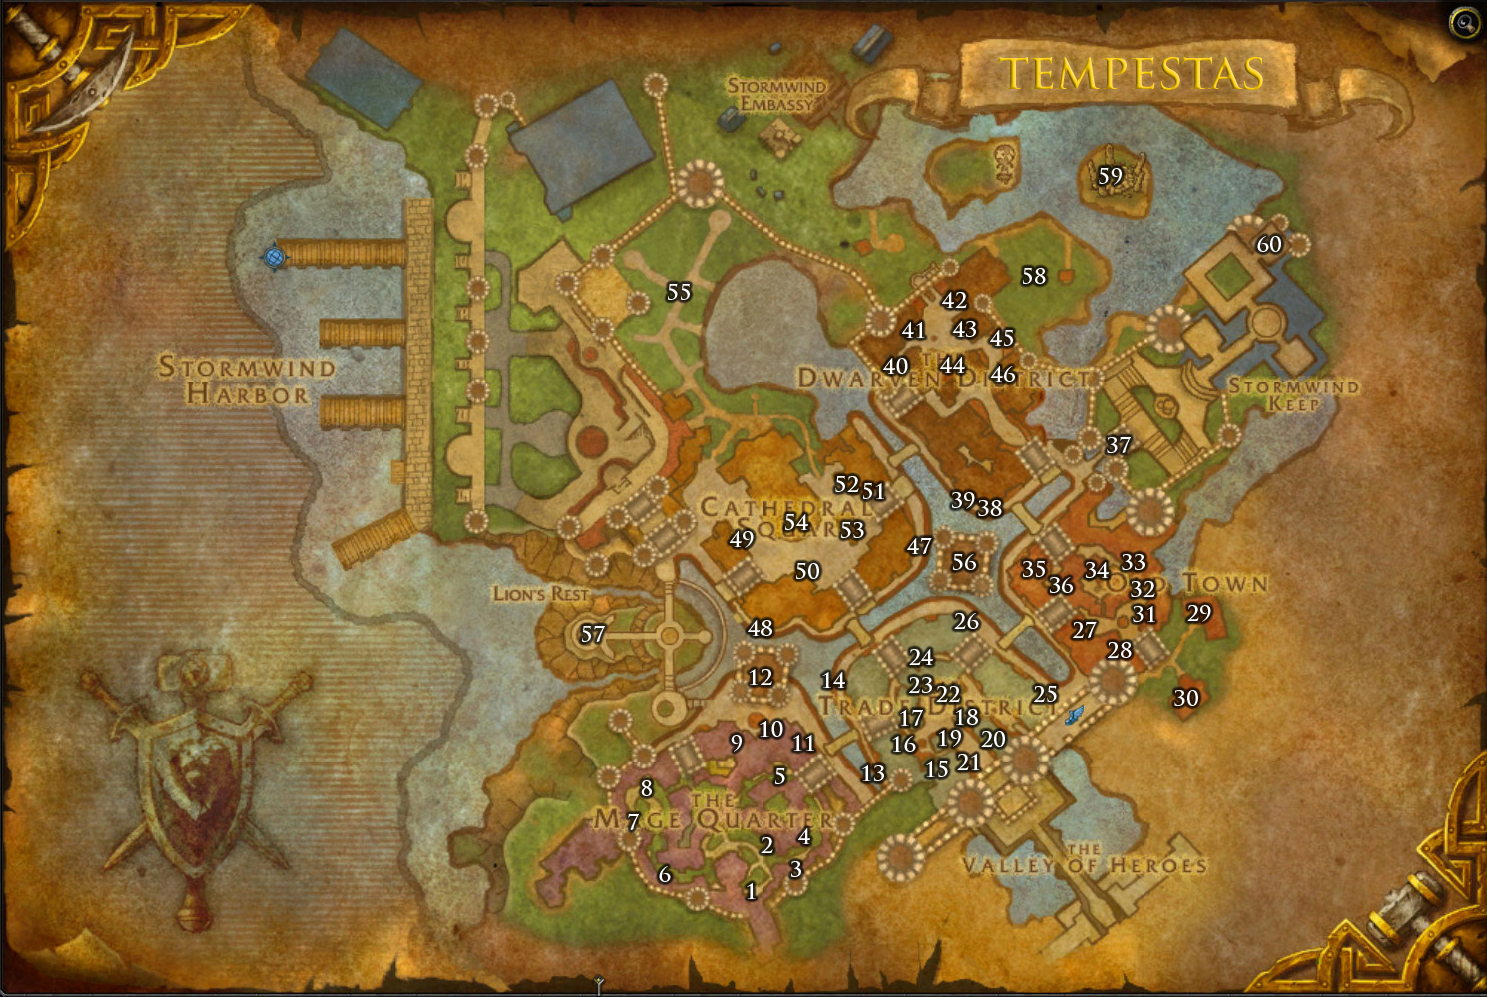
\includegraphics[width=\linewidth]{img/Tempestas_labeled.jpg}
	
	{\begin{multicols}{3}
		\begin{enumerate}
			\item The Blue Recluse (Tavern)
			\item Larson Clothiers
			\item Alchemy Needs
			\item Duncan's Textiles
			\item Tempestas Staves
			\item Ancient Curios
			\item The Slaughtered Lamb (Pub)
			\item Pyrotechnics
			\item The Scribe of Tempestas
			\item Academy of Arcane Arts
			\item Cordell's Enchanting
			\item Tempestas Prison
			\item Gallina Winery
			\item Canal Tailor and Fit shop
			\item Tempestas Counting House (Bank)
			\item The Gilded Rose (Inn)
			\item Tempestas Trade House
			\item Everyday Merchandise
			\item Pestle's Apothecary
			\item Trias' Cheese
			\item Tempestas Visitor's Center
			\item Weller's Arsenal
			\item Lionheart Armory
			\item Barbara's Barbor
			\item Fragrant Flowers
			\item Denman Family Jewelers
			\item The Protective Hide
			\item Champion's Hall
			\item SI:7
			\item Command Center
			\item Limited Immunity (Armors)
			\item Honest Blades
			\item Pig \& Whistle Tavern
			\item Heavy Handed Weapons
			\item The Silver Shield
			\item Thane's Boots
			\item Tempestas Keep
			\item Pott's Plates
			\item The Shady Lady
			\item Stonehand Mining
			\item Auction House
			\item Royal Bank of Tempestas
			\item The Golden Keg (Tavern)
			\item Engineering Ward
			\item Deeprun Tram
			\item Hunters Hovel
			\item Ol' Emmas
			\item The Three Winds
			\item Just Maces
			\item Rightous Plates
			\item The Argent Dawn
			\item City Hall
			\item Orphanage
			\item Cathedral
			\item Graveyard
			\item Maximum Security
			\item Varian Wrynn Memorial
			\item Audrey Burnhep
			\item Earthshrine
			\item Royal Library
		\end{enumerate}
	\end{multicols}}
\end{center}

\subsection{Tempestas Hierarchy}

Within Tempestas, there is a hierarchy of power and rule. The Hierarchy of who is in charge is as follows.
\begin{enumerate}
	\item King and Queen.
	\begin{enumerate}
		\item The King is at the head of the City. He controls the military and decisions of the Nobles. His family is at the head of the government and economic system in Tempestas.
	\end{enumerate}
	\item Royal Advisory.
	\begin{enumerate}
		\item Royal Guard. The Royal Guard is the Kings personal protection for him and his family. These guards are specially trained in matters of combat and intelligence.
		\item Royal Council. The Royal Council is a group of wise men and advisors that the King uses in making decisions pertaining to the times. These include Daniel the Prophet, Kinsey the military advisor, Turelyon the religious advisor, and Nicholas the economic advisor. 
	\end{enumerate}
	\item Nobles
	\begin{enumerate}
		\item Nobles. The Nobles are the rich elite that control different sub-sections of the city. There are seven Nobles in total which each essentially control a different part of the city.
		\begin{enumerate}
			\item Sir Francis Lancelot. He is head over the Trade district. He is the big economic power in Tempestas as he controls teh trade markets and the banking system. He oversees a Nobles vault within the bank which is like a security deposit system for rare and valuable items.
			\item Saint Palagius the Wise. This is the Noble overhead of the Cathedral Square and all of its businesses. This includes the Cathedral and Graveyard of Tempestas.
			\item Delgore Zuba de Hut. This is the Noble overhead of the Storm wind Harbor. He has control over trade and harbor security. When the city is in lock down, the only way to enter or leave is through his permission or the Kings. 
			\item Gimley Bronzebeard. This is the Noble over the Dwarven District. He is head of the Brawler's Guild which is an underground club where the black market is located and run.
			\item Others
		\end{enumerate}
		\item Noble Families. Right below the Nobles, the Noble families have a large amount of power just through affiliation with the Nobles.
		\item Noble Guards. Since the Nobles have a vast amount of power and money, they have their own guards and watch over different parts of the cities. The King is ahead of all of these troops in times of National security but in general they are lead by the Noble above them.
		\item Noble Councils. The Nobles generally have their own councils and workers directly under them.
	\end{enumerate}
	\item Tempestas Officials.
	\begin{enumerate}
		\item Mayor. This is the head of civil affairs. He has minor control over laws and resources used throughout the city.
		\item District leaders. These are generally appointed by the Nobles (indirectly) through a 'democratic' voting system. They are in charge of affairs relating to the businesses throughout each sector.
		\item Trade leaders. These are the head business men in each division (trade, religion, crafting, etc).
		\item Tempestas Guards. These are normal guards appointed to be on duty throughout the city. Much like a police force.
	\end{enumerate}
	\item Shop keepers.
	\item Citizens.
\end{enumerate}

\subsection{Brawlers Guild}

The Brawlers guild is a secret underground club that was created by black market leaders and allowed to exist by the Nobles. Any corrupt business dealings will generally go on here as it is privately guarded with Mercenary bouncers. Entrance to the Brawlers Guild requires a scroll of approval (Brawlers pass) with the signatures of the Brawler officials. These passes are hard to obtain and generally extremely expensive. Within the Brawlers guild is an underground sand arena where fights and battles are waged. There is a custom orchestra playing music for the fights and bets are placed on the battles. The champion of the arena (Jay Maul) is essentially Darth Maul from Star Wars only wields a duel bladed stave with electrical capabilities. He is an agile fighter who makes many small attacks quickly in succession and is hard to hit.









\section{The Statu Peninsula}

The Statu peninsula (commonly referred to as just Statu) is largly un-mapped area. As the name suggests, Statu is a peninsula that cannot be accessed from foot to the north. It contains very dense forestation and mountainous regions to the northern area that are not possible to travel through. The south is colonized by Aurushire where a small number of people settle. There are generally a small number of visitors to Statu, save those who are trading and working with the mines to the East of Aurushire. The best way to access Statu is through the Aurushire port.

To the West of Aurushire, there is a large forest that is significantly less dense than the northern regions. To the north of this is very dense un-explored forest and mountainous regions. Directly north of Aurushire is The Pluvian Forest. This region is not very often visited. Strange occurances pertaining to what some call 'strange spatial events' occur in The Pluvian Forest which generally ward off visitors. To the southeast of Aurushire, there is a hostile tribe of river Naga which attack travelers and visitors on sight. Because of this, the area to the southeast and the forest regions to the East of Aurushire are unexplored. What is known of this region is that there is a large valley that leads from the Naga camps into the mountain/forest region.

\section{Aurushire}

Aurushire (also commonly referred to as Goldshire) is a small village located on the southern end of the Statu peninsula. Just East of Aurushire is a large mountain containing mine shafts used for gold mining. It is not well known, other by those who work in the mines, but strange things happen within these mines where mined gold will spontaneously be regrown after being removed from the mines. This phenomenon is where Aurushire (Goldshire) retreived its name from and is thought to be related to the spacial occurrences reported in The Pluvian Forest. 

\begin{center}
	\includegraphics[width=\linewidth]{img/maps/Aurushire.png}
	
	{\textbf{Aurushire:} To the south is the sea entrance. In the northwest is a secluded area where Baba Lives. To the northeast is a secluded area where Belmod lives. The North path leads to The Pluvian Forest and the West path leads to Rem Silva. The East side of the village is the location of Auru Convallis and the Naga camps are on the southeast side of the area leading into the eastern forest.}
\end{center}

\subsection{NPC's}

Aurushire is full of NPC characters. Many of them are just normal workers or village folk, however some serve an important purposes. Some of them include the innkeeper, the Pandaren Brothers, the village watchers and the shopkeepers.

\begin{monsterbox}{Arryn}
	\begin{hangingpar}
		\textit{Halfling Wizard, Neutral Good}
	\end{hangingpar}
	\dndline%
	\basics[%
	armorclass = 17,
	hitpoints  = 172,
	speed      = 40 ft
	]
	\dndline%
	\stats[
	STR = \stat{12}, % This stat command will autocomplete the modifier for you
	DEX = \stat{12},
	CON = \stat{16},
	INT = \stat{20},
	WIS = \stat{18},
	CHA = \stat{18}
	]
	\dndline%
	\details[%
	% If you want to use commas in these sections, enclose the
	% description in braces.
	% I'm so sorry.
	languages = {Common, Elvish, Dwarvish, Gnomish, Halfling, Orc, Pandaren},
	challenge = 10
	]
	\dndline%
	\begin{monsteraction}[Mystical Senses]
		If a target tries to deceive you, it must make a DC19 deception saving throw.
	\end{monsteraction}	
	\begin{monsteraction}[Water sight]
		You can see clearly up to two miles over water.
	\end{monsteraction}
	\monstersection{Actions}
	\begin{monsteraction}[Bladesinger: Extra Attack]
		You can attack twice on your turn.
	\end{monsteraction}
	\begin{monsteraction}[Hold Monster]
		A creature you can see within 90 feet must succeed on a wisdom saving throw or be paralyzed for 1 minute. Target can make a wisdom saving throw at the end of each of it's turns to end the spell.
	\end{monsteraction}
	\begin{monsteraction}[Magic Jar Master]
		Allows Arryn to use Magic Jar on a nearby jar instantly and without being in a jar himself.
	\end{monsteraction}
	\begin{monsteraction}[Magic Jar]
		Long description, look it up.
	\end{monsteraction}
	\monstersection{Description/Information}
	Arryn is the first NPC most encounter when entering Aurushire from sea. He is the watcher of the ports and lives on a small farm right at docks where all sea traffic enters from.
\end{monsterbox}

\begin{center}
	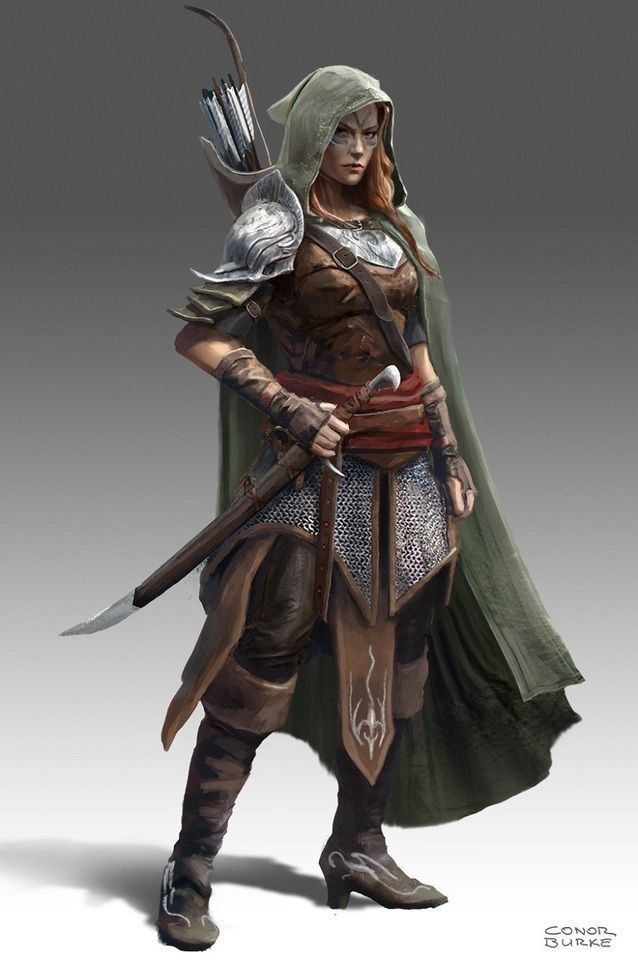
\includegraphics[width=0.27\linewidth]{img/NPCs/Tamina.jpg} 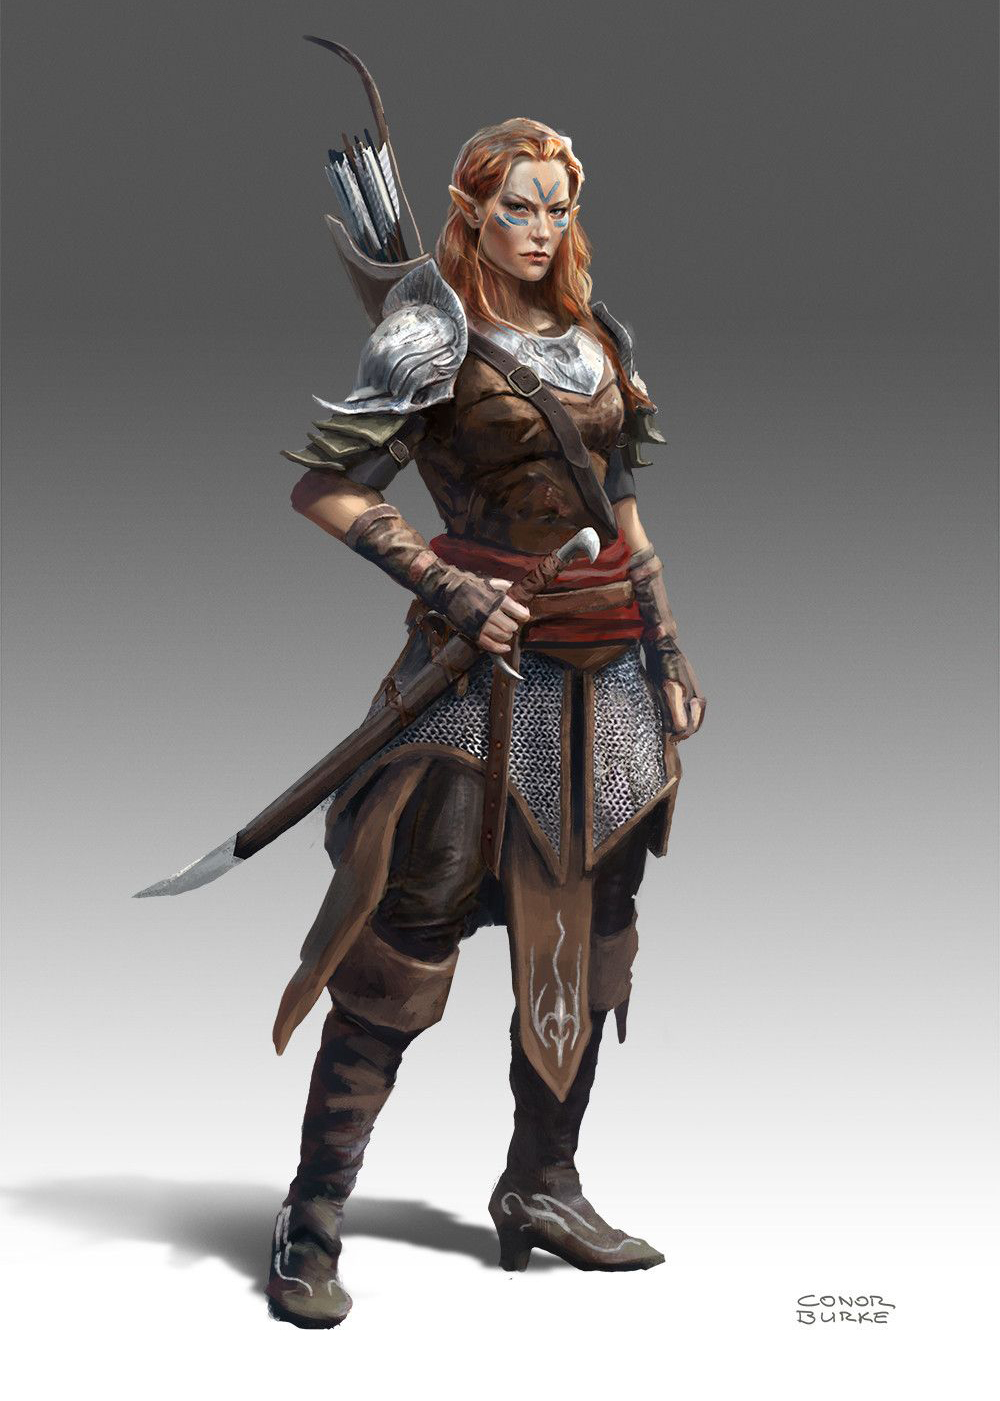
\includegraphics[width=0.29\linewidth]{img/NPCs/Tamina2.jpg} 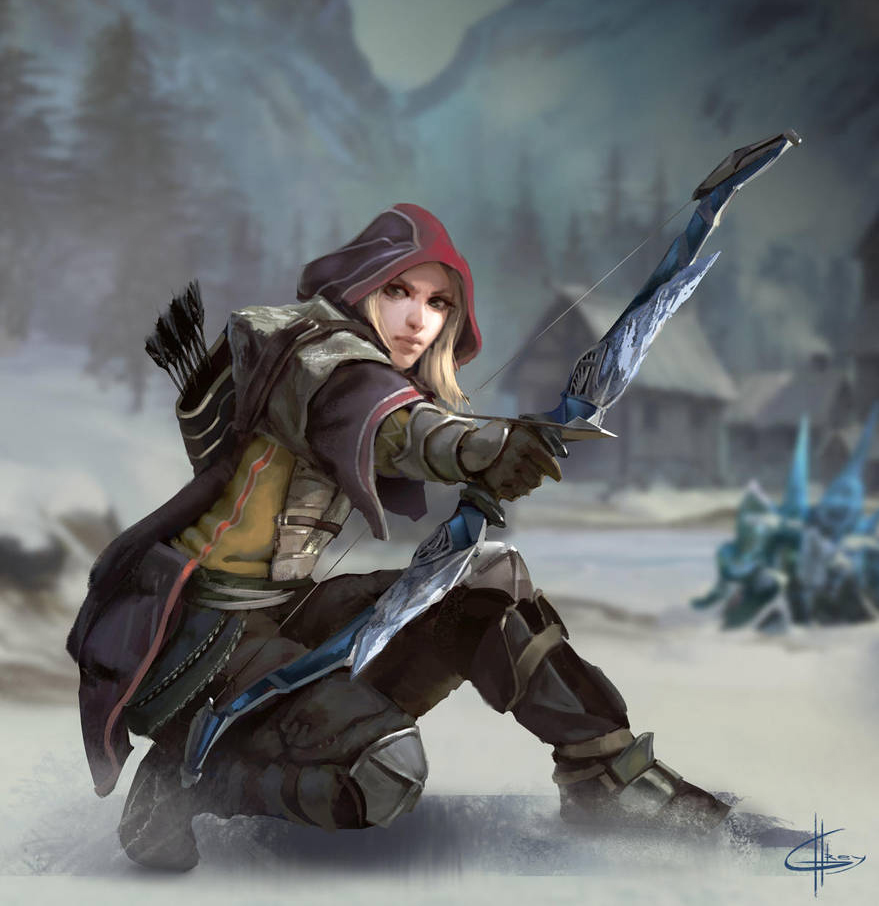
\includegraphics[width=0.395\linewidth]{img/NPCs/Tamina3.jpg}
\end{center}

\begin{monsterbox}{Tamina}
	\begin{hangingpar}
		\textit{Human Ranger, Neutral Good}
	\end{hangingpar}
	\dndline%
	\basics[%
	armorclass = 18,
	hitpoints  = 154,
	speed      = 40 ft
	]
	\dndline%
	\stats[
	STR = \stat{18}, % This stat command will autocomplete the modifier for you
	DEX = \stat{18},
	CON = \stat{12},
	INT = \stat{14},
	WIS = \stat{13},
	CHA = \stat{11}
	]
	\dndline%
	\details[%
	% If you want to use commas in these sections, enclose the
	% description in braces.
	% I'm so sorry.
	languages = {Common, Elvish, Pandaren},
	challenge = 10
	]
	\dndline%
	\begin{monsteraction}[Mystical Senses]
		If a target tries to deceive you, it must make a DC19 deception saving throw.
	\end{monsteraction}	
	\begin{monsteraction}[Water sight]
		You can see clearly up to two miles over water.
	\end{monsteraction}
	\begin{monsteraction}[Bladesinger: Extra Attack]
		You can attack twice on your turn.
	\end{monsteraction}
	\monstersection{Actions}
	\begin{monsteraction}[Paralytic Dart]
		Hit: +3. A creature you can see within 90 feet must succeed on a wisdom saving throw or be paralyzed for 1 minute.
	\end{monsteraction}
	\begin{monsteraction}[Aimed Shot]
		Hit: +6. Damage: 3d6 + 4 piercing damage. You pull our your longbow and fire a single arrow aimed precisely where you choose. 
	\end{monsteraction}
	\begin{monsteraction}[Scatter Shot]
		Hit: +6. Damage 1d6 + 2 piercing damage per arrow. You grasp up to 4 arrows and mount them in your bow. You must roll hit for each arrow you attempt to fire and can choose up to 4 targets for the various arrows.
	\end{monsteraction}
	\begin{monsteraction}[Blade Slash]
		Hit: +5. Damage 2d6 + 3 slashing damage per arrow. You pull our your silvered short sword and make a melee attack against the target.
	\end{monsteraction}

	\monstersection{Description/Information}
	Tamina is a watcher of Aurushire. She trains under Arryn and the Stormstout brothers and spends the majority of her time roaming the outskirts of the town keeping watch for dangers or new occurrences in the area.
\end{monsterbox}

\begin{center}
	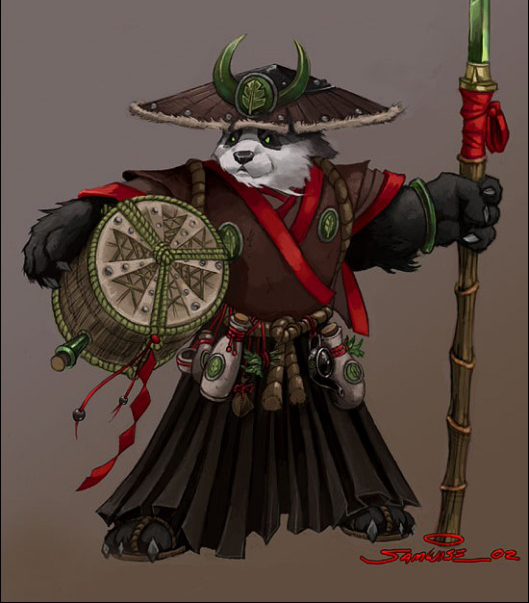
\includegraphics[width=0.39\linewidth]{img/WoW/chen.jpg} 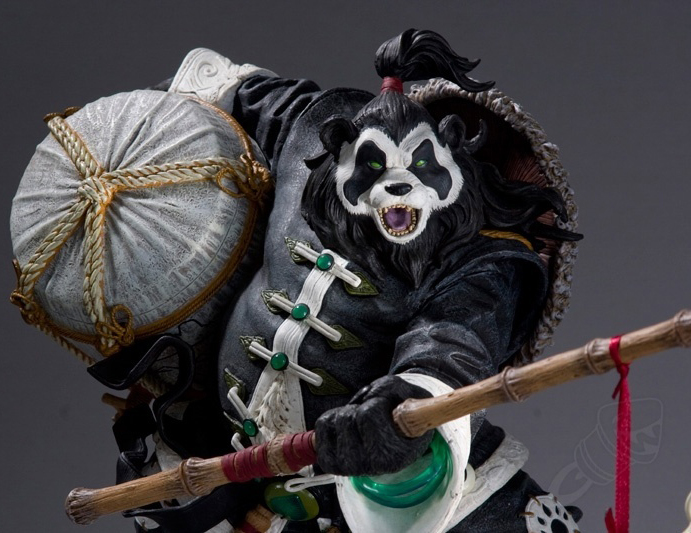
\includegraphics[width=0.575\linewidth]{img/WoW/153930.jpg}
\end{center}

\begin{monsterbox}{Chen Stormstout}
	\begin{hangingpar}
		\textit{Pandaren Monk, Neutral Good}
	\end{hangingpar}
	\dndline%
	\basics[%
	armorclass = 17,
	hitpoints  = 172,
	speed      = 40 ft
	]
	\dndline%
	\stats[
	STR = \stat{18}, % This stat command will autocomplete the modifier for you
	DEX = \stat{20},
	CON = \stat{16},
	INT = \stat{12},
	WIS = \stat{12},
	CHA = \stat{18}
	]
	\dndline%
	\details[%
	% If you want to use commas in these sections, enclose the
	% description in braces.
	% I'm so sorry.
	languages = {Common, Elvish, Dwarvish, Gnomish, Halfling, Orc, Pandaren},
	challenge = 10
	]
	\dndline%
	\begin{monsteraction}[Joint lock]
		You can put a creature in a joint lock when attacking. Remove 1d6 damage from the attack and instead roll 1d20 to decide on how severe the joint lock is. 
		
		1-3: The joint lock fails. 
		
		4-14: You pop a joint briefly out of place causing the enemy to have disadvantage on their next attack.
		
		15-19: You dislocate the targeted limb, causing the opponent to not be able to use it until set (which can be done via an action on their turn). You can choose to roll less if desired.
		
		20: You tear the tendons holding a limb on, causing it to become useless until healed. You can choose to roll less if desired.
	\end{monsteraction}
	\begin{monsteraction}[Pressure Point Mastery]
		You can target a creatures pressure points when attacking. Remove 1d6 damage from the attack and instead roll 1d20 to decide how accurate the points are hit. 
		
		1-3: The pressure points fail. 
		
		4-14: You hit a target in a precious spot causing them great discomfort. They must roll attack rolls at disadvantage next round.
		
		15-19: The target becomes stunned for one round of combat. You can choose to roll less if desired.
		
		20: The target becomes completely paralyzed. You can choose to roll less if desired.
	\end{monsteraction}
	\monstersection{Actions}
	\begin{monsteraction}[Pandaren Nimbleness: Extra Attack]
		You can attack twice on your turn.
	\end{monsteraction}
	\begin{monsteraction}[Melee]
	This is a normal un-armed melee attack: +6 to hit. Deals 3d6 +5 damage.
	\end{monsteraction}
	\begin{monsteraction}[Armed Melee]
		This is a normal melee attack using a weapon. Depending on the weapon, it can add damage to the Melee attack. Spear/staff: +6 damage, Sword: +4 damage, Hammer/Axe: +2 damage.
	\end{monsteraction}

	\monstersection{Description/Information}
	Chen Stormstout runs the Aurushire Pub. He spends his time wandering the nearby regions for herbs and ingredients to make the perfect brews. He also studies martial arts with his brothers. He focuses on pressure points and joint locks and studies a more fluid form of combat.
\end{monsterbox}

\begin{center}
	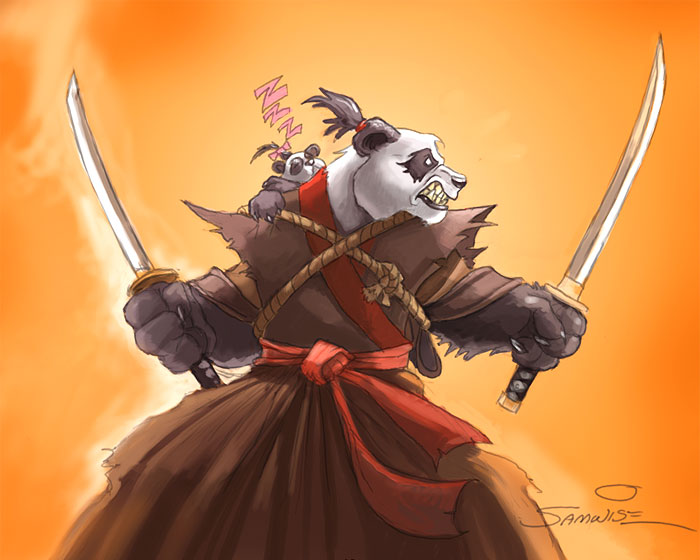
\includegraphics[width=0.60\linewidth]{img/WoW/ekron.jpg} 
\includegraphics[width=0.375\linewidth]{img/WoW/twopandare.jpg}
\end{center}

\begin{monsterbox}{Ekron Stormstout}
	\begin{hangingpar}
		\textit{Pandaren Barbarian, Neutral Good}
	\end{hangingpar}
	\dndline%
	\basics[%
	armorclass = 17,
	hitpoints  = 172,
	speed      = 50 ft
	]
	\dndline%
	\stats[
	STR = \stat{20}, % This stat command will autocomplete the modifier for you
	DEX = \stat{18},
	CON = \stat{18},
	INT = \stat{12},
	WIS = \stat{12},
	CHA = \stat{16}
	]
	\dndline%
	\details[%
	% If you want to use commas in these sections, enclose the
	% description in braces.
	% I'm so sorry.
	languages = {Common, Elvish, Dwarvish, Gnomish, Halfling, Orc, Pandaren},
	challenge = 10
	]
	\dndline%
	\begin{monsteraction}[Fury of Blows]
		If you have two swords, you can furiously attack your opponent without them being able to block. You can sacrifice any number of 1d6's from the attack roll to destroy an item the opponent has on them.
	\end{monsteraction}	
	\monstersection{Actions}
	\begin{monsteraction}[Pandaren Nimbleness: Extra Attack]
		You can attack twice on your turn.
	\end{monsteraction}
	\begin{monsteraction}[Melee]
	This is a normal un-armed melee attack: +6 to hit. Deals 3d6 +5 damage.
	\end{monsteraction}
	\begin{monsteraction}[Armed Melee]
		This is a normal melee attack using a weapon. Depending on the weapon, it can add damage to the Melee attack. Spear/staff: +4 damage, Sword: +6 damage, Hammer/Axe: +2 damage.
	\end{monsteraction}
	\monstersection{Description/Information}
	Ekron, like his brothers, also studies martial arts.He focuses on agility and movements to quickly take down his opponents with a fierce and fast form of combat. He is the keeper of the Aurushire Quarries and leads the mining operations. He found a small panda in the forest one day and has been cherishing it ever since as a friend and companion.
\end{monsterbox}

\begin{center}
	
\includegraphics[width=0.48\linewidth]{img/WoW/mishnah.jpg} 		
\includegraphics[width=0.48\linewidth]{img/WoW/mishna.jpg}
\end{center}

\begin{monsterbox}{Mishnah Stormstout}
	\begin{hangingpar}
		\textit{Pandaren, Neutral Good}
	\end{hangingpar}
	\dndline%
	\basics[%
	armorclass = 17,
	hitpoints  = 172,
	speed      = 30 ft
	]
	\dndline%
	\stats[
	STR = \stat{20}, % This stat command will autocomplete the modifier for you
	DEX = \stat{18},
	CON = \stat{18},
	INT = \stat{12},
	WIS = \stat{16},
	CHA = \stat{18}
	]
	\dndline%
	\details[%
	% If you want to use commas in these sections, enclose the
	% description in braces.
	% I'm so sorry.
	languages = {Common, Elvish, Dwarvish, Gnomish, Halfling, Orc, Pandaren},
	challenge = 10
	]
	\dndline%
	\begin{monsteraction}[Thunderous Blow]
		You can sacrifice 2d6 on an attack roll to instead deal 1d4 thunderous damage to all enemies within 15 feet of the blow you deal.
	\end{monsteraction}	
	\monstersection{Actions}
	\begin{monsteraction}[Pandaren Nimbleness: Extra Attack]
		You can attack twice on your turn.
	\end{monsteraction}
	\begin{monsteraction}[Melee]
		This is a normal un-armed melee attack: +6 to hit. Deals 3d6 +5 damage.
	\end{monsteraction}
	\begin{monsteraction}[Armed Melee]
		This is a normal melee attack using a weapon. Depending on the weapon, it can add damage to the Melee attack. Spear/staff: +2 damage, Sword: +4 damage, Hammer/Axe: +6 damage.
	\end{monsteraction}
	\monstersection{Description/Information}
	Mishnah Stormstout is the Aurushire Blacksmith. He spends his time collecting rocks and forging precious metals found in his brothers mine. He also studies martial arts but tends more towards a body building focus and overpowers his foes through brute strength.
\end{monsterbox}

\begin{center}
	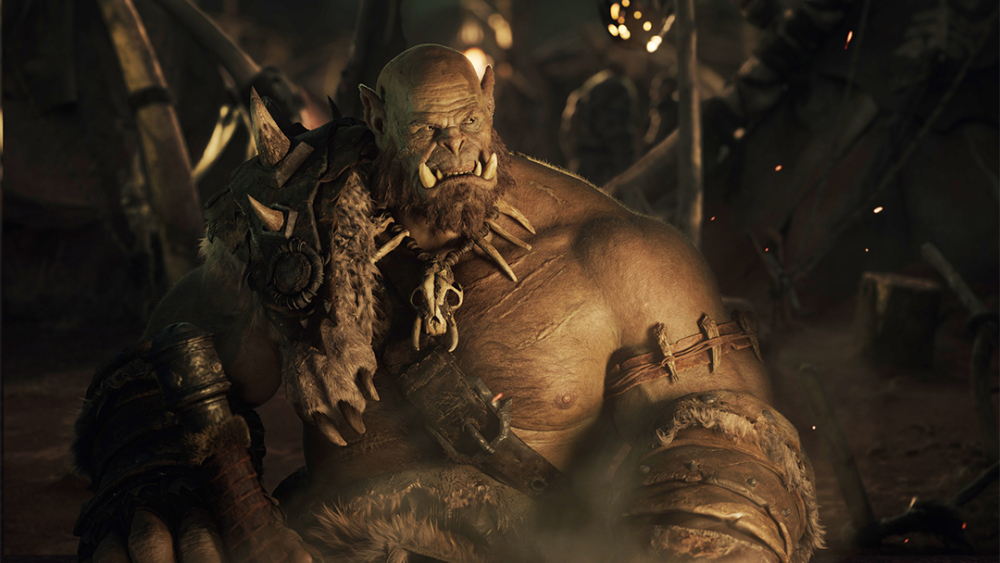
\includegraphics[width=0.7\linewidth]{img/WoW/bob.jpg}
\end{center}

\begin{monsterbox}{Bob}
	\begin{hangingpar}
		\textit{Orcish Barbarian, Neutral Good}
	\end{hangingpar}
	\dndline%
	\basics[%
	armorclass = 17,
	hitpoints  = 151,
	speed      = 30 ft
	]
	\dndline%
	\stats[
	STR = \stat{20}, % This stat command will autocomplete the modifier for you
	DEX = \stat{18},
	CON = \stat{17},
	INT = \stat{16},
	WIS = \stat{15},
	CHA = \stat{13}
	]
	\dndline%
	\details[%
	% If you want to use commas in these sections, enclose the
	% description in braces.
	% I'm so sorry.
	languages = {Common, Dwarvish, Orc},
	challenge = 9
	]
	\dndline%
	\begin{monsteraction}[Experienced Pain]
		Bob has seen some things. He can ignore any major wounds or hindrances that would effect his combat. He can fight full power until his last breath. This is due to his combat experience and many near death experiences.
	\end{monsteraction}	
	\begin{monsteraction}[Battle Master]
		Bob can quickly pick up and adapt to using most weapons, gaining proficiency with any new weapons after using them.
	\end{monsteraction}	
	\monstersection{Actions}
	\begin{monsteraction}[Combat experience: Extra Attack]
		You can attack twice on your turn.
	\end{monsteraction}
	\begin{monsteraction}[Melee]
		This is a normal un-armed melee attack: +6 to hit. Deals 2d6 +5 damage.
	\end{monsteraction}
	\begin{monsteraction}[Throwing Axe]
		Bob carries 4 throwing axes that he can hurl towards an enemy. +5 to hit. 3d6 +2 damage. Range: 40 ft.
	\end{monsteraction}
	\monstersection{Description/Information}
	
\end{monsterbox}


\subsection{The Inn of the Prancing Pony}

This is the inn located in Aurushire. The innkeeper is named Artemisia who is kind of like the grandmother of the small village. 

\subsection{Tracey's Armory}

Tracey's Armory is the armor shop in Aurushire. The shopkeeper is Tiberias Tracey, who is one of the great grandchildren of the original shop's builder. This shop contains simple and custom armor pieces that are created for all who are willing to pay or friends of Tiberias. 

\subsection{Bob's Guns}

Bob's Guns is a relatively newly built shop. The majority of what is sold here is ranged weapons. Due to the effects of the Pluvian Forest, Bob (the storekeeper) discovered a weapon laying in the wild on someones corpse. He was able t reverse engineer approximately how it worked and has been creating 'guns' ever since. Unfortunately he used all of the bullets on the original design, but he was able to examine the weapon itself and deduce a process to recreate a similar mechanism, His own designs are not as well made as the original discovery, but they are slowly improving over time. Bob also sells spears, throwing stars, darts, bows and more.

\subsection{Stormstout Blacksmith}

This is the village blacksmith that is run by one of the Stormstout brothers (Mishnah). The blacksmith is one of the watchers of the village and most influential members. Mishnah is also friends with everyone else in the village and generally his services are needed by almost all of the members.

\begin{commentbox}{Working in the Mines}
	The players are able to work in the blacksmith for either gold or skills. The players can work for either 20 gold a day or they can work for one of the following skills.
	\begin{description}
		\item[7 day:] Apprentice smithy: They can be taught how to make basic smithing items. Their success on the items will depend on a d20 roll.
		\item[1 month:] Novice smithy: They can be taught how to make novice smithing items and possibly enhance other items. Their success on the items will depend on a d20 roll.
		\item[1 year:] Master smithy: They can be taught how to make master smithing items and enhance other smithed items. Their success on the items will depend on a d20 roll.
	\end{description}
\end{commentbox}

\subsection{Stormstout Pub}

This is the village brewery which is unlike any brewery anywhere else. The brewery is run by one of the Stormstout brothers (Chen). Chen ha ssome of the most unique brews of anywhere else in Orilla. This is primarily due to the ingredients and herbs that he has found throughout the nearby forests. Chen is one of the friendliest people in Aurushire and most people go to him with their issues or thoughts. He is generally a sociable person and many people hang out at his Brewery/Pub in their free time. Chen is also one of the watchers of the village and most influential members.

\begin{commentbox}{Working in the Mines}
	The players are able to work in the pub for either gold or skills. The players can work for either 20 gold a day or they can work for one of the following skills.
	\begin{description}
		\item[7 day:] Apprentice brewer: They can be taught how to make brews from new ingredients they find. Their success on the brews will depend on a d20 roll.
		\item[1 month:] Novice brewer: They can be taught how to make Novice brews and potions from new ingredients they find. Their success on the brews will depend on a d20 roll.
		\item[1 year:] Master brewer: They can be taught how to make master brews, potions, and elixirs from new ingredients they find. Their success on the brews will depend on a d20 roll.
	\end{description}
\end{commentbox}

\subsection{Stormstout Quarries}

The Stormstout Quarries are the mines that reside to the East of Aurushire. The mines are run by one of the Stormstout brothers (Ekron). Ekron is a strong military leader and one of the most influential members of Aurushire. The mines are known for their unique regrowth of some of the ores within them. It is believed that these occurrences are as a result of effects on the region by the Pluvian Forest. The quarries will pay any willing workers with a part of their earnings. Ekron is one of the watchers of the village.

\begin{commentbox}{Working in the Mines}
	The players are able to work in the mines for gold. The payout for gold is dealt daily and events occurring in the mines can be determined by rolling a d20. The mines are generally safe, but can be dangerous if you are not paying attention. Before working in the mines the players must agree to the terms of work which include replacing equipment destroyed by their use.
	
	\begin{description}
		\item[1:] Disaster struck while you were in the mine. You end up fracturing a limb (making it un-usable until healed) and breaking some equipment that you rented. You have to repay for the equipment which totals 300g. If the player does not have this they go in debt.
		\item[2:] Disaster struck while you were in the mine. breaking some equipment that you rented. You have to repay for the equipment which totals 300g. If the player does not have this they go in debt.
		\item[3:] Disaster struck while you were in the mine. breaking some equipment that you rented. You have to repay for the equipment which totals 100g. If the player does not have this they go in debt.
		\item[4:] You were unable to make much progress in the mine. You're tired, exhausted, and have not come out with any profits. You only have to pay a renting fee for the equipment you borrowed which totals 10g. If the player does not have this they go in debt.
		\item[5-6:] You have a sluggish day in the mine. You break even walking away with no profit.
		\item[7-10:] You worked a descent shift. You struck gold (literally) and tried to mine it all well. Your cut for the day is 10g.
		\item[11-14:] You worked a descent shift. You struck gold (literally) and tried to mine it all well. Your cut for the day is 25g.
		\item[15-16:] You worked a great shift. You struck gold (literally) mined it all well. Your cut for the day is 50g.
		\item[17:] You worked a great shift. You struck gold (literally) mined it all well. Your cut for the day is 100g.
		\item[18:] You worked a perfect shift. You struck gold (literally) mined it all perfectly. Your cut for the day is 200g.
		\item[19:] You worked a perfect shift. You struck gold (literally) mined it all perfectly. Your cut for the day is 400g.
		\item[20:] You worked a perfect shift. You struck gold (literally) and also stumbled across a new rare gemstone and mined it all perfectly. Your cut for the day is 1000g.
	\end{description}
\end{commentbox}

\subsection{Library of Lysanias}

The village has a library that is open to all. There are a number of people who spend a lot of time here and maintain it but for the most part it is open and there is no main keeper. The library is public and contains mostly learning material and books written by previous and past villagers. Many of the books found in this place are old and have not been touched in years. Similarly, the writing style of the books is very old and many of them are simply dense materials with no index or table of contents. The books in this library can range from story to history to fiction. There are some engineering and science books but none that would pertain to enchanting or magic. All of the magic books have been taken to Baba's Tower.

\begin{commentbox}{Books in the Library of Lysanias}
	Some of the books that can be found in this library are as follows.
	\begin{itemize}
		\item A book of prophecies. This book simply says `prophecies' on the cover. It is dense.
		\item A 65 volume set on night elves. These books explain the history of elves in this area and others. 
		\item Fables of a Guardian past. These books contain information pertaining to the legends of the Celestial Guard, written as if a fictional story.
		\item Legends of three Dragons. These contain stories pertaining to three dragons living in the lands of a sacred forest.
		\item Weapons of the black witch. Pertaining to stories of ancient weapons created for various dark servants.
		\item A 25 volume set on artifacts. These books discuss various artifacts that were created and hidden through time.
		\item Legends of the past kings.
		\item Fables of Lysanias. Books outlying the adventures of Lysanias. 
	\end{itemize}
\end{commentbox}







\section{Rem Silva}

Rem Silvia is the name of the Forest that is located to the West of Aurushire. This forest, along with The Pluvian Forest often experiences strange spacial phenomenon. Unlike The Pluvian Forest, temporal phenomenon have also commonly been reported as occurring in this region. The occurrences of these random phenomenon do not appear marginally as often or as strong as in The Pluvian Forest which makes this region of particular interest to experienced hunters.

The same strange effects that can occur in the Pluvian forest can also occur here in Rem Silva only less frequently. As a DM, you can periodically roll a 1d20 to see if any of the irregular effects from The Pluvian Forest will also occur here. Subtract 5 from each DC throw to see if the effects occur in this region.

This area is full of a large number of creatures, from large spiders, to night elfs. Due to the trinity stone effects, many creatures not belonging to this region also appear here. 

\begin{commentbox}{Random Encounters}
	At any time, a party traveling through this area could run into a creature. To determine a random encounter you can roll 1d100 and choose what the party will encounter. If the roll is odd, choose a miscellaneous creature from Appendix A of the monster manual (page 317-337 in monster manual, roll 1d20 to decide page of creature to choose), otherwise if the roll is even, choose from the table below. Similarly, Page 97 of Xanathars may be useful for creating random encounters.
	\begin{description}
		\item[1-10:] Displacer Beast
		\item[11-20:] Basilisk
		\item[21-25:] Dinosaur (page 79-80 of monster manual)
		\item[26-30:] Unicorn (page 294 of monster manual)
		\item[31-40:] Night elf(s)
		\item[41-45:] Ettin (page 132 of monster manual)
		\item[46-50:] troll (page 291 of monster manual)
		\item[51-55:] Galeb Duhr (page 139 of monster manual)
		\item[56-60:] Yeti (page 305 of monster manual)
		\item[61-65:] Ghost (page 147 of monster manual)
		\item[66-70:] Hook Horrer (page 189 of monster manual)
		\item[71-75:] Griffon (page 174 of monster manual)
		\item[76-80:] Hippogriff (page 184 of monster manual)
		\item[81-85:] Hell Hound (page 182 of monster manual)
		\item[86-90:] Jackalwere (page 193 of monster manual)
		\item[91-95:] Homunculus (page 188 of monster manual)
		\item[96-99:] Treant (page 289 of monster manual)
		\item[100:] Mythical Beast
	\end{description}
\end{commentbox}

\subsection{NPC's/Modified Creatures}

\begin{center}
	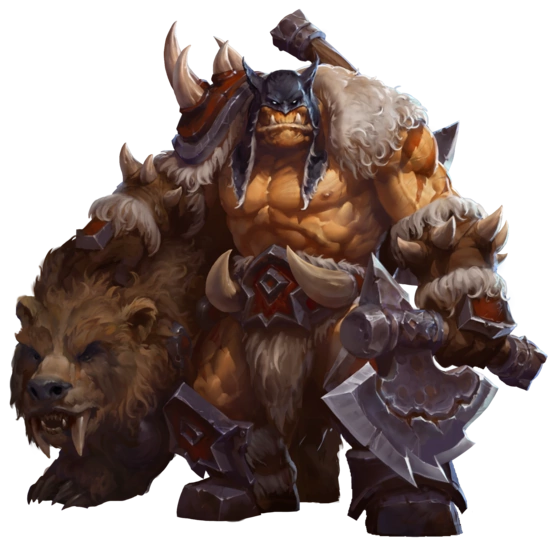
\includegraphics[width=0.38\linewidth]{img/WoW/Rexxar2.png}
	\includegraphics[width=0.6\linewidth]{img/WoW/Rex.jpg}
\end{center}
\begin{monsterbox}{Rexxar}
	\begin{hangingpar}
		\textit{Large humanoid, unaligned}
	\end{hangingpar}
	\dndline%
	\basics[%
	armorclass = 21,
	hitpoints  = 457,
	speed      = 50 ft
	]
	\dndline%
	\stats[
	STR = \stat{27}, % This stat command will autocomplete the modifier for you
	DEX = \stat{14},
	CON = \stat{25},
	INT = \stat{16},
	WIS = \stat{15},
	CHA = \stat{19}
	]
	\dndline%
	\details[%
	% If you want to use commas in these sections, enclose the
	% description in braces.
	% I'm so sorry.
	savingthrows = {Dex +9, Con +14, Wis +9, Char +11},
	skills = {Perception +16, Stealth +9},
	senses = {darkvision 90 ft., passive perception 26},
	languages = {common, Dwarvish},
	challenge = 21 (27500 XP)
	]
	\dndline%
	\begin{monsteraction}[Legendary Resistance (3/day)]
		If Rexxar fails a saving throw, he can choose to succeed instead.
	\end{monsteraction}	

	
	\monstersection{Actions}
	\begin{monsteraction}[Multiattack]
		Rexxar can make three attacks, one with each Axe and one with another weapon he has.
	\end{monsteraction}
	\begin{monsteraction}[Axe knock]
		Melee Weapon Attack: +15 to hit, reach 10ft., one target. Hit: 15 (2d6 + 8) bludgeoning damage. The target must succeed a DC 15 strength check or be knocked unconscious.
	\end{monsteraction}
	\begin{monsteraction}[Axe Slash]
		Melee Weapon Attack: +15 to hit, reach 10ft., one target. Hit: 18 (3d6 + 8) slashing damage.
	\end{monsteraction}
	\begin{monsteraction}[Axe Throw]
		Ranged Weapon Attack: +15 to hit, reach 35 ft., one target. Hit: 19 (2d10 + 8) piercing damage.
	\end{monsteraction}
	\begin{monsteraction}[Legendary Throw]
		Rexxar Drops one of his large Axes and hurls the other through the air with all his strength. This attack consumes all three of Rexxars attacks. Ranged Weapon Attack: +15 to hit, reach 45 ft., one target. Hit: 60 (10d10+10) damage. This attack will deal triple damage to a target that does not see it coming. Rexxar also gains 1 level of exhaustion from this attack.
	\end{monsteraction}
	\monstersection{Legendary Action}
	Rexxar can take 3 legendary actions per day.
	\begin{monsteraction}[Unbroken Will.]
		Rexxar Can use his sheer strength to free himself from any immobilizing effect or device.
	\end{monsteraction}
	\monstersection{Description/Information}
	Rexxar has lived in Rem Silva his entire life. He gets his strength from when he was a boy. Due to the effects of the energy stone on a fountain he drank out of, he is blessed with extraordinary strength. Along with his life of successful hunts, Rexxar has legendary strength and wit.
\end{monsterbox}

\begin{monsterbox}{Bella (Rexxar's Pet)}
	\begin{hangingpar}
		\textit{Large Beast (Bear), unaligned}
	\end{hangingpar}
	\dndline%
	\basics[%
	armorclass = 14,
	hitpoints  = 84,
	speed      = 40 ft
	]
	\dndline%
	\stats[
	STR = \stat{22}, % This stat command will autocomplete the modifier for you
	DEX = \stat{12},
	CON = \stat{18},
	INT = \stat{4},
	WIS = \stat{15},
	CHA = \stat{9}
	]
	\dndline%
	\details[%
	% If you want to use commas in these sections, enclose the
	% description in braces.
	% I'm so sorry.
	skills = Perception +5,
	senses = {passive perception 15},
	challenge = 3 (700XP)
	]
	\dndline%
	\begin{monsteraction}[Keen Smell]
		The bear has advantage on Wisdom (Perception) checks that rely on smell.
	\end{monsteraction}	
	
	\monstersection{Actions}
	\begin{monsteraction}[Multiattack]
		The bear makes two attacks: one with its bite and one with its claws.
	\end{monsteraction}
	\begin{monsteraction}[Bite]
		Melee Weapon Attack: +7 to hit, reach 5 ft., one target. Hit: 9 (ld8 + 5) piercing damage.
	\end{monsteraction}
	\begin{monsteraction}[Claws]
		Melee Weapon Attack: +7 to hit, reach 5 ft ., one target. Hit: 12 (2d6 + 5) slashing damage.
	\end{monsteraction}
	\monstersection{Description/Information}
		Bella was saved as a cub by Rexxar. Her parents were attacked by an ancient dinosaur that appeared due to the space stone. Rexxar raised Bella and trained her to follow commands and she has stuck by his side ever since.
\end{monsterbox}


\begin{monsterbox}{Ancient Displacer Beast}
	\begin{hangingpar}
		\textit{Large Monstrosity, lawful evil}
	\end{hangingpar}
	\dndline%
	\basics[%
	armorclass = 16,
	hitpoints  = 170,
	speed      = 40 ft
	]
	\dndline%
	\stats[
	STR = \stat{19}, % This stat command will autocomplete the modifier for you
	DEX = \stat{16},
	CON = \stat{17},
	INT = \stat{7},
	WIS = \stat{13},
	CHA = \stat{9}
	]
	\dndline%
	\details[%
	% If you want to use commas in these sections, enclose the
	% description in braces.
	% I'm so sorry.
	senses = {darkvision 70 ft., passive perception 12},
	challenge = 6 (700XP)
	]
	\dndline%
	\begin{monsteraction}[Avoidance]
		If the displacer beast is subjected to an effect that allows it to make a saving throw to take only half damage, it instead takes no damage if it succeeds on the saving throw and only half damage if it fails.
	\end{monsteraction}	
	\begin{monsteraction}[Dark Stealth]
		The beast can succeed any stealth check against a creature that is not aware of it's existence/location.
	\end{monsteraction}	
	\begin{monsteraction}[Displacement]
		The displacer projects a magical illusion that makes it appear to be standing near its actual location, causing attack tolls against it to have disadvantage. Due to the space stone effect on this beast, this trait is always active.
	\end{monsteraction}	
	\monstersection{Actions}
	\begin{monsteraction}[Multiattack]
		The displacer can make two attacks with its tentacles. 
	\end{monsteraction}
	\begin{monsteraction}[Tentacle]
		Melee Weapon Attack: +6 to hit, reach 10 ft., one target. Hit: 10 (2d6 +4) bludgeoning damage plus 6 (2d6) piercing damage.
	\end{monsteraction}
	\begin{monsteraction}[Shear of Space]
		Melee Weapon Attack: +6 to hit, reach 100 ft., one target. Hit: 10 (2d6 +4) bludgeoning damage plus 3 (1d6) piercing damage. The creature reaches it's claw through space and attacks a target at range (It can only do this because of the space stone existence in a nearby region).
	\end{monsteraction}	
	\monstersection{Description/Information}
	These creatures roam Rem Silva, but due to the effect of the space stones, they can fade in and out of reality. As opposed to the normal displacer beasts of the region, the Ancient displacer beast can voluntarily phade out of reality at will when under 40 hp.
\end{monsterbox}


\begin{monsterbox}{Displacer Beast}
	\begin{hangingpar}
		\textit{Large Monstrosity, lawful evil}
	\end{hangingpar}
	\dndline%
	\basics[%
	armorclass = 13,
	hitpoints  = 85,
	speed      = 40 ft
	]
	\dndline%
	\stats[
	STR = \stat{18}, % This stat command will autocomplete the modifier for you
	DEX = \stat{15},
	CON = \stat{16},
	INT = \stat{6},
	WIS = \stat{12},
	CHA = \stat{8}
	]
	\dndline%
	\details[%
	% If you want to use commas in these sections, enclose the
	% description in braces.
	% I'm so sorry.
	senses = {darkvision 60 ft., passive perception 11},
	challenge = 3 (700XP)
	]
	\dndline%
	\begin{monsteraction}[Avoidance]
		If the displacer beast is subjected to an effect that allows it to make a saving throw to take only half damage, it instead takes no damage if it succeeds on the saving throw and only half damage if it fails.
	\end{monsteraction}	
	\begin{monsteraction}[Displacement]
		The displacer projects a magical illusion that makes it appear to be standing near its actual location, causing attack tolls against it to have disadvantage. Due to the space stone effect on this beast, this trait is always active.
	\end{monsteraction}	
	\monstersection{Actions}
	\begin{monsteraction}[Multiattack]
		The displacer can make two attacks with its tentacles. 
	\end{monsteraction}
	\begin{monsteraction}[Tentacle]
		Melee Weapon Attack: +6 to hit, reach 10 ft., one target. Hit: 7 (1d6 +4) bludgeoning damage plus 3 (1s6) piercing damage.
	\end{monsteraction}	
	\monstersection{Description/Information}
	These creatures roam Rem Silva, but due to the effect of the space stones, they can fade in and out of reality (at random but not at will).
\end{monsterbox}

\begin{monsterbox}{Basilisk}
	\begin{hangingpar}
		\textit{Medium Monstrosity, unaligned}
	\end{hangingpar}
	\dndline%
	\basics[%
	armorclass = 15,
	hitpoints  = 52,
	speed      = 20 ft
	]
	\dndline%
	\stats[
	STR = \stat{16}, % This stat command will autocomplete the modifier for you
	DEX = \stat{8},
	CON = \stat{15},
	INT = \stat{2},
	WIS = \stat{8},
	CHA = \stat{7}
	]
	\dndline%
	\details[%
	% If you want to use commas in these sections, enclose the
	% description in braces.
	% I'm so sorry.
	senses = {darkvision 60 ft., passive perception 9},
	challenge = 3 (700XP)
	]
	\dndline%
	\begin{monsteraction}[Petrifying gaze]
		If a creature starts its turn within 30 ft and they can see each other, the basilisk can force a DC12 constitution saving throw (If the basilisk isn't incapacitated). One a fail, the greature begins to turn to stone and is restrained. It must repeat the saving throw at the end of its next turn. On a success, the effect ends. On a failure,  the creature is petrified until freed by the greater restoration spell or other magic.
		
		A creature not surprised can avert its eyes to avoid the saving throw at the start of its turn. If it does it cannot see the basilisk until the start of its next turn, when it can avert its eyes again. If it looks at the basilisk in the meantime, it must immediately make the save.
		
		If the basilisk sees it's reflection in bright light, it targets itself with it's gaze. 
	\end{monsteraction}	
	\begin{monsteraction}[Irregular Stone Skin]
		As a byproduct of the energy stones effect on the basilisk, enemies must roll at disadvantage if the basilisk succeeds a DC 12 strength save. Upon a failed attack agaisnt the basilisk, its skin hardens to absorb the impact of an attack.
	\end{monsteraction}	
	\monstersection{Actions}
	\begin{monsteraction}[Bite]
		Melee Weapon Attack: +5 to hit, reach 5 ft., one target. Hit 10 (2d6+3) piercing damage plus 7(2d6) poison damage.
	\end{monsteraction}
	\monstersection{Description/Information}
	These creatures roam around Rem Silva. Due to the effect of the energy stone, these creatures can be small or large with their stats adjusted accordingly. 
\end{monsterbox}

\begin{monsterbox}{Bullywug}
	\begin{hangingpar}
		\textit{Medium humanoid, neutral evil}
	\end{hangingpar}
	\dndline%
	\basics[%
	armorclass = {15 (hide armor, shield)},
	hitpoints  = 11 (2d8 +2),
	speed      = {20 ft, swim 40 ft.}
	]
	\dndline%
	\stats[
	STR = \stat{12}, % This stat command will autocomplete the modifier for you
	DEX = \stat{12},
	CON = \stat{13},
	INT = \stat{7},
	WIS = \stat{10},
	CHA = \stat{7}
	]
	\dndline%
	\details[%
	% If you want to use commas in these sections, enclose the
	% description in braces.
	% I'm so sorry.
	skills = {stealth +3}
	senses = {passive perception 10},
	challenge = 1/4 (50 XP)
	]
	\dndline%
	\begin{monsteraction}[Amphibious]
		The bullywug can breathe air and water.
	\end{monsteraction}	
	\begin{monsteraction}[Swamp Camouflage]
		The bullywug has advantage on Dexterity (stealth) checks made to hide in swampy terrain.
	\end{monsteraction}	
	\begin{monsteraction}[Standing Leap]
		The bullywug's long jump is up to 20 ft. and its high jump is up to 10 ft.
	\end{monsteraction}	

	\monstersection{Actions}
	\begin{monsteraction}[Multiattack]
		The bullywig makes two melee attacks: one with it's bite and one with its spear.
	\end{monsteraction}
	\begin{monsteraction}[Bite]
		Melee weapon attack: +3 to hit, reach 5 ft., one target. Hit: 3(1d4 +1) bludgeoning damage.
	\end{monsteraction}
	\begin{monsteraction}[Spear]
		Melee or ranged weapon attack: +3 to hit, reach 5 ft. or range 20/60., one target. Hit 4(1d6 +1) piercing damage or 5(1d8) piercing damage if used with two hands to make a melee attack. 
	\end{monsteraction}
	\monstersection{Description/Information}
		These creatures inhabit the river running through the center of Rem Silva. They have a camp at the southern end just before the opening to the sea.
\end{monsterbox}

\begin{monsterbox}{Ankylosaurus}
	\begin{hangingpar}
		\textit{Huges Beast, unaligned}
	\end{hangingpar}
	\dndline%
	\basics[%
	armorclass = 15,
	hitpoints  = 68,
	speed      = 30 ft
	]
	\dndline%
	\stats[
	STR = \stat{19}, % This stat command will autocomplete the modifier for you
	DEX = \stat{11},
	CON = \stat{15},
	INT = \stat{2},
	WIS = \stat{12},
	CHA = \stat{5}
	]
	\dndline%
	\details[%
	% If you want to use commas in these sections, enclose the
	% description in braces.
	% I'm so sorry.
	senses = {passive perception 11},
	challenge = 3 (700XP)
	]
	\dndline%	
	\monstersection{Actions}
	\begin{monsteraction}[Tail]
		Melee Weapon Attack: +7 to hit, reach 10 ft. one target. Hit: 18 (4d6 +4) bludgeoning damage. If the target is a creature, it must succeed a DC14 strength saving throw of be knocked prone.
	\end{monsteraction}
	\monstersection{Description/Information}
		Because od the time stone, prehistoric creatures like this can appear throughout Rem Silva.
\end{monsterbox}

\begin{monsterbox}{Night Elf Elite Warrior}
	\begin{hangingpar}
		\textit{Medium humanoid (elf), unaligned}
	\end{hangingpar}
	\dndline%
	\basics[%
	armorclass = 18,
	hitpoints  = 71,
	speed      = 30 ft
	]
	\dndline%
	\stats[
	STR = \stat{13}, % This stat command will autocomplete the modifier for you
	DEX = \stat{18},
	CON = \stat{14},
	INT = \stat{11},
	WIS = \stat{13},
	CHA = \stat{12}
	]
	\dndline%
	\details[%
	% If you want to use commas in these sections, enclose the
	% description in braces.
	% I'm so sorry.
	savingthrows = {Dex +7, Con +5, Wis +4},
	skills = {Perception +4, Stealth +10},
	senses = {darkvision 120 ft., passive perception 14},
	languages = {Elvish, undercommon, common},
	challenge = 5 (1800 XP)
	]
	\dndline%
	\begin{monsteraction}[Fey Ancestry]
		The elf has advantage on saving throws against being charmed, and magic can't put the elf to sleep.
	\end{monsteraction}	
	\begin{monsteraction}[Innate Spellcasting]
		The elfs spellcasting ability is Charisma (spell save DC 12). It can innately cast the following spells, requiring no material components:
		\begin{enumerate}
			\item At will: dancing lights
			\item 1/day each: darkness ,faerie fire , levitate (self only)
		\end{enumerate}
	\end{monsteraction}	
	\begin{monsteraction}[Sunlight Sensitivity]
		While in sunlight, the elf has disadvantage on attack rolls, as well as on Wisdom (Perception) checks that rely on sight.
	\end{monsteraction}	
	
	\monstersection{Actions}
	\begin{monsteraction}[Multiattack]
		The elf can make two shortsword attacks.
	\end{monsteraction}
	\begin{monsteraction}[Shortsword]
		Melee Weapon Attack: +7 to hit, reach 10ft., one target. Hit: 7 (ld6 + 4) piercing damage plus 10 (3d6) poison damage.
	\end{monsteraction}
	\begin{monsteraction}[Hand Crossbow]
		Ranged Weapon Attack: +7 to hit, range 30/120 ft ., one target. Hit: 7 (ld6 + 4) piercing damage, and the target must succeed on a DC 13 Constitution saving throw or	be poisoned for 1 hour. If the saving throw fails by 5 or more,	the target is also unconscious while poisoned in this way. The target wakes up if it takes damage or if another creature takes an action to shake it awake.
	\end{monsteraction}
	\monstersection{Reactions}
	\begin{monsteraction}[Parry]
		the elf adds 3 to its AC against one melee attack that would hit it. To do so, the elf must see the attacker and be
		wielding a melee weapon.
	\end{monsteraction}
	\monstersection{Description/Information}
		The night elves roam Rem Silva hiding in plain sight. They are the watchers of the forest. 
\end{monsterbox}

\begin{monsterbox}{Night Elf Elite Marksman}
	\begin{hangingpar}
		\textit{Medium humanoid (elf), unaligned}
	\end{hangingpar}
	\dndline%
	\basics[%
	armorclass = 18,
	hitpoints  = 71,
	speed      = 30 ft
	]
	\dndline%
	\stats[
	STR = \stat{12}, % This stat command will autocomplete the modifier for you
	DEX = \stat{19},
	CON = \stat{14},
	INT = \stat{11},
	WIS = \stat{13},
	CHA = \stat{13}
	]
	\dndline%
	\details[%
	% If you want to use commas in these sections, enclose the
	% description in braces.
	% I'm so sorry.
	savingthrows = {Dex +7, Con +5, Wis +4},
	skills = {Perception +4, Stealth +10},
	senses = {darkvision 120 ft., passive perception 14},
	languages = {Elvish, undercommon, common},
	challenge = 5 (1800 XP)
	]
	\dndline%
	\begin{monsteraction}[Fey Ancestry]
		The elf has advantage on saving throws against being charmed, and magic can't put the elf to sleep.
	\end{monsteraction}	
	\begin{monsteraction}[Innate Spellcasting]
		The elfs spellcasting ability is Charisma (spell save DC 12). It can innately cast the following spells, requiring no material components:
		\begin{enumerate}
			\item At will: dancing lights
			\item 1/day each: darkness ,faerie fire , levitate (self only)
		\end{enumerate}
	\end{monsteraction}	
	\begin{monsteraction}[Sunlight Sensitivity]
		While in sunlight, the elf has disadvantage on attack rolls, as well as on Wisdom (Perception) checks that rely on sight.
	\end{monsteraction}	
	
	\monstersection{Actions}
	\begin{monsteraction}[Multiattack]
		The elf can make two longbow attacks.
	\end{monsteraction}
	\begin{monsteraction}[Shortsword]
		Melee Weapon Attack: +7 to hit, reach 10ft., one target. Hit: 7 (ld6 + 4) piercing damage plus 10 (3d6) poison damage.
	\end{monsteraction}
	\begin{monsteraction}[Longbow]
		Ranged Weapon Attack: +7 to hit, range 30/120 ft ., one target. Hit: 10 (2d6 + 4) piercing damage, and the target must succeed on a DC 13 Constitution saving throw or	be poisoned for 1 hour. If the saving throw fails by 5 or more,	the target is also unconscious while poisoned in this way. The target wakes up if it takes damage or if another creature takes an action to shake it awake.
	\end{monsteraction}
	\monstersection{Reactions}
	\begin{monsteraction}[Skillful Avoidance]
		the elf adds 3 to its AC against one attack that would hit it. To do so, the elf must see the attacker and be
		wielding a longbow.
	\end{monsteraction}
	\monstersection{Description/Information}
	The night elves roam Rem Silva hiding in plain sight. They are the watchers of the forest. 
\end{monsterbox}

%\begin{monsterbox}{Template}
%	\begin{hangingpar}
%		\textit{Medium Monstrosity, unaligned}
%	\end{hangingpar}
%	\dndline%
%	\basics[%
%	armorclass = 15,
%	hitpoints  = 52,
%	speed      = 20 ft
%	]
%	\dndline%
%	\stats[
%	STR = \stat{16}, % This stat command will autocomplete the modifier for you
%	DEX = \stat{8},
%	CON = \stat{15},
%	INT = \stat{2},
%	WIS = \stat{8},
%	CHA = \stat{7}
%	]
%	\dndline%
%	\details[%
%	% If you want to use commas in these sections, enclose the
%	% description in braces.
%	% I'm so sorry.
%	senses = {passive perception 9},
%	challenge = 3 (700XP)
%	]
%	\dndline%
%	\begin{monsteraction}[Petrifying gaze]
%		
%	\end{monsteraction}	
%	
%	\monstersection{Actions}
%	\begin{monsteraction}[Bite]
%		
%	\end{monsteraction}
%	\monstersection{Description/Information}
%\end{monsterbox}

\section{The Pluvian Forest}

\subsubsection{About the Region}

The Pluvian Forest is the name of the forest that is located to the North of Aurushire. The forest is known for strange spacial occurrences happening within it. Those who travel into The Pluvian Forest do not generally return or will return very confused or changed.

\subsubsection{Unique Forest Dynamics}

The Pluvian Forest is largely effected by the contents of the Spati Aethereu Thalamun (Aethereu). It is a normal forest in itself but it's close proximity to Aethereu makes this region dangerous. The forest is heavily affected by the space stone such that visitors can be lost for weeks while only traveling through a few days worth of terrain. Similarly, the time stone has the strongest connection to the space stone and thus has a great influence on the area. Often, travelers find the days lasting longer or shorter than usual. The energy stone has an effect on this region which amplifies the effect of the other two stones.

\begin{commentbox}{Irregular Days}
	As a byproduct of the time stone effecting the region, often the days find themselves to be shortened or lengthened due to the time stone effect from Aethereu. As a DM, you can determine periodically if there is any effect on travelers by rolling a 1d20 and succeeding a DC11 time throw. If failed, roll a 1d20 to determine the effect on the party.
	\hline
	\begin{description}
		\item[1:] Party transported 1 year into the future. 
		\item[2:] Party transported 3 months into the future. This may induce a season change. 
		\item[3:] Party transported 2 weeks into the future. This may induce a temperature change.
		\item[4-5:] Party transported 1 day into the future. 
		\item[6-7:] Party transported 5 hours into the future. 
		\item[8-10:] Party transported 1 hour into the future. 
		\item[11-13:] Party transported 1 hour into the past. 
		\item[14-15:] Party transported 5 hours into the past. 
		\item[16-17:] Party transported 1 day into the past. 
		\item[18:] Party transported 2 weeks into the past. This may induce a temperature change. 
		\item[19:] Party transported 3 months into the past. This may induce a season change. 
		\item[20:] Party transported 1 year into the past. 
	\end{description}
\end{commentbox}

\begin{commentbox}{Irregular Creatures}
	As a byproduct of the time stone working in conjunction with the space stone effecting the region, often creatures of objects of strange origin can appear in the area. As a DM, you can determine periodically if there is any effect on travelers by rolling a 1d20 and succeeding a DC13 space-time throw. If failed, roll a 1d20 to determine the effect on the party.
	\hline
	\begin{description}
		\item[1:] A prehistoric dinosaur appears in a nearby area.
		\item[2:] A long known-to-be extinct creature appears in a nearby area.
		\item[3:] A creature not native to this area appears in a nearby area.
		\item[4:] An ancient item appears in a nearby area.
		\item[5-6:] A creature native to the area appears behind the party.
		\item[7-10:] An item owned by a player vanishes and teleports to a location shortly behind them on their path.
		\item[11-14:] An item owned by a player vanishes and teleports to a location shortly ahead of them on their path.
		\item[15-16:] A creature native to the area appears ahead of the party.
		\item[17:] A futuristic item appears in a nearby area.
		\item[18:] A creature not native to this area appears in the nearby area.
		\item[19:] A natural creature that has never been seen before appears in the area.
		\item[20:] A robotic creature appears in the area.
	\end{description}
\end{commentbox}

\begin{commentbox}{Irregular Movement}
	As a byproduct of the space stone effecting the region, often the part finds themselves being moved around to different areas or places they have been before. As a DM, you can determine periodically if there is any effect on travelers by rolling a 1d20 and succeeding a DC15 space throw. If failed, roll a 1d20 to determine the effect on the party.
	\hline
	\begin{description}
		\item[1:] One member of the party is teleported to the entrance of The Pluvian Forest.
		\item[2:] The party members are teleported to a random location in The Pluvian Forest (chosen by the DM or completely random).
		\item[3:] The party is instantly moved to the last place they teleported from. If they have not been teleported yet, nothing will happen.
		\item[4:] Roll a DC12 save. Upon failing, the party is teleported to Rem Silvia.
		\item[5-6:] An object being carried by a member of the party is teleported just behind them on their path.
		\item[7-8:] The party is turned around.
		\item[9- 10:] The party is teleported to a place just ahead of where they weree. If they pass a DC15 perception check they will know they have moved. 
		\item[11-12:] The party is teleported to a place they recently were. If they pass a DC15 perception check they will know they have moved. The party may see tracks left by them which would lead them back to where they were.
		\item[13-14:] The party is turned around.
		\item[15-16:] An object being carried by a member of the party is teleported just ahead of them on their path. 
		\item[17:] Roll a DC12 save. Upon failing, the party is teleported to Aurushire.
		\item[18:] The party is instantly moved to the last place they teleported from. If they have not been teleported yet, nothing will happen.
		\item[19:] The party members are teleported to a random location in The Pluvian Forest (chosen by the DM or completely random).
		\item[20:] One member of the party is teleported to the end of The Pluvian Forest.
	\end{description}
\end{commentbox}

\begin{commentbox}{Irregular Energy}
	As a byproduct of the energy stone effecting the region, often creatures are either not as strong as they seem or have extraordinary strength. As a DM, you can determine periodically if there is any effect on travelers by rolling a 1d20 and succeeding a DC11 energy throw. If failed, roll a 1d20 to determine the effect on the party.
	\hline
	\begin{description}
		\item[1-5:] A member of the party acquires a level of exhaustion.
		\item[6:] A member of the party loses a spell slot.
		\item[7:] A member of the party loses 10 HP.
		\item[8-10:] A creature has all of its strength sapped and is very easy to defeat.
		\item[11-15:] Objects or areas of the forest glow and irradiate magical power. This can be trees, a stream, a pond, creatures, the ground, the path, or anything else. 
		\item[16-17:] A creature of the forest is bestowed with extraordinary strength (depending on party condition).
		\item[18:] A member of the party gains 10 HP. 
		\item[19:] A member of the party gains a missing spell slot. 
		\item[20:] A member of the party loses a level of exhaustion.
	\end{description}
\end{commentbox}

\subsubsection{Navigating The Pluvian Forest}

In order to successfully navigate through The Pluvian Forest and find Aethereu, the party must follow a simple set of instructions, while not getting turned around by the irregular occurrences. These set of instructions may be given to the party in a variety of ways (see below). 

\begin{commentbox}{Successful Navigation}
	\begin{description}
		\item[Guidence of Time] When nature calls, you must follow it's guidance. You must follow the hoot of the owls and the sounds of the wolves.
		\item[Guidence of Space] The correct path points to the stars. Follow the hills up and not down.
		\item[Guidence of Energy] The forest seeks to distract. Avoid illusions created by the energy stone.
		\item[Guidence of the Trinity] When the trinity is broken, search for the missing link. When two of the rules above are broken, look for the third to act.
	\end{description}
\end{commentbox}

\subsection{NPC's}

All of the creatures that can appear in The Pluvian forest are the same as those of Rem Silva Except the night elves and Rexxar/Bella. Similarly, the party can encounter a number of various other creatures.

\subsection{Encounters and Discoveries}

Throughout the forest, many things can happen to the party including visions/dreams, strange occurrences, interesting discoveries, and more.

\begin{commentbox}{Fountain of Plasma}
	Within the forest there exists a circular three layer fountain. It is rather large and contains a thick glowing liquid. The liquid is clear like water, but also warm to the touch and flows slowly in reverse as it would in a normal fountain. The fountain has an extreme index of refraction and so it appears as though it is only a few inches deep. However, the players can reach their entire arms into the fountain if they so choose.
	
	Within the fountain is a scroll that can only be acquired by reaching deep into the fountain and grabbing some of the water then pulling their hand out. If they grab the deep water, a scroll will materialize from the liquid as it hits the air. The scroll that materializes is known as the Scroll of Myrd.
\end{commentbox}


\begin{commentbox}{Scroll of Myrd}
	The scroll of Myrd has a sweet aroma. The scroll itself contains an indecipherable language that appears to have a different character for each letter. this is unreadable by any sense. The key to understanding the scroll is to eat the scroll. If the scroll is eaten, it is bitter to the taste (worse than pure cranberries). When consumed, the devourer will gain the understanding of the scroll.	
\end{commentbox}


\begin{commentbox}{Riddle of Myrd}
	The Riddle of Myrd is a piece of information that Baba has. She will give it to the party to aid on their journey through the Pluvian Forest.
	\begin{quote}
		Within the Pluvian realm, one must focus at the helm.
		
		For the puzzle of the forest, fall hidden in the water crest.
		
		There the scroll of exit may be found, and escape contained in what is round.
		
		The soul of your being in danger now, the secret way, you must find how.
		
		To save the soul, one must devour the scroll.
		
		For the knowledge of what's next, is contained within its text.
		
		And the power of this word, is greater than that heard.
		
		To escape this place, and win the race.
	\end{quote}
\end{commentbox}


\subsection{Trinity Dragons}

Within the Pluvian Forest are three Dragons. Each one created by Myrddin and containing an item to help obtain and control the Trinity Stones. 

\begin{commentbox}{Infernalous}
	Infernalous is a large dragon created by Myrddin. The dragon is very old and extremely intelligent. This dragon is modeled after lava and fire and his abilities are in accordance with such. This dragon has poor eyesight, but can smell sweat and blood. He can control minor aspects of space by moving the earth around him and even phasing through the earth around him. He can relocate lava from deep within the earth and use it as a weapon himself.
	
	\begin{center}
	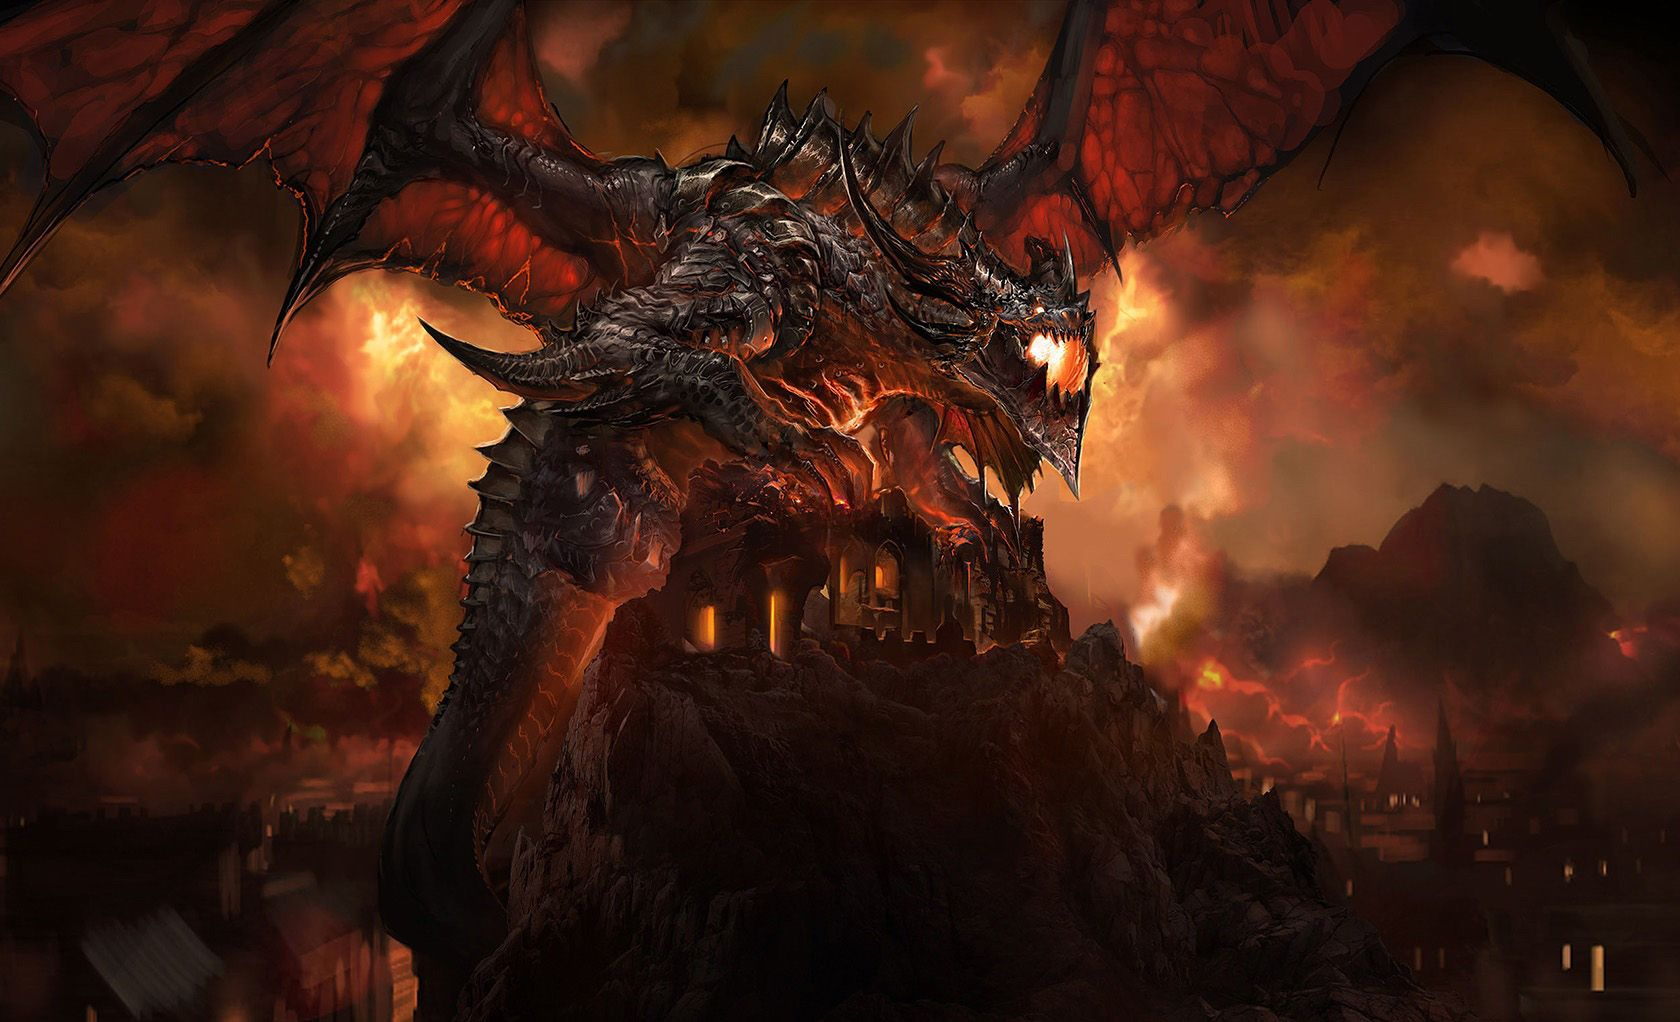
\includegraphics[width=0.7\linewidth]{img/WoW/deathwing.jpg}
	\end{center}

	Within the cavern of Infernalous contains one of three magical rings created by Myrddin, a red-gemmed ring. There are also other treasures that can be found within the cavern such as armor and shields from fallen foes who have traveled into the cavern. 

	\begin{center}
	
\includegraphics[width=0.7\linewidth]{img/maps/infernalous.jpg}
	\end{center}
\end{commentbox}

\begin{commentbox}{Aquaeleous}
	Aquaeleous is a large dragon created by Myrddin. The dragon is very old and extremely intelligent. This dragon is modeled after life and the lifeless and his abilities are in accordance with such. This dragon has poor hearing and sight, but can feel vibrations of the earth for those around. He can control minor aspects of matter by changing the materials around them and changing the states of matter.
	
	\begin{center}
	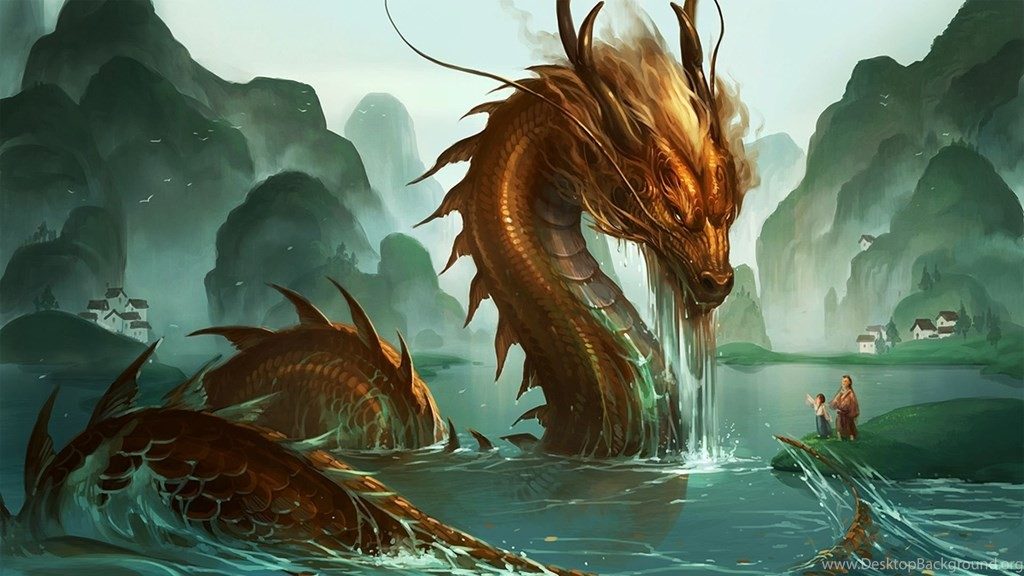
\includegraphics[width=0.7\linewidth]{img/waterdragon.jpg}
	\end{center}
	
	Within the cavern of Aquaeleous contains one of three magical rings created by Myrddin, a yellow-gemmed ring. There are also other treasures that can be found within the cavern such as staves, bows and other items from fallen foes who have traveled into the cavern. 
	
	\begin{center}
	
\includegraphics[width=0.7\linewidth]{img/maps/aquaeleous.jpg}
	\end{center}
\end{commentbox}


\begin{commentbox}{Crystalleous}
	Crystalleous is a large dragon created by Myrddin. The dragon is very old and extremely intelligent. This dragon is modeled after water and spirits and his abilities are in accordance with such. This dragon has poor hearing and sight, but can feel vibrations of the earth for those around. He can control minor aspects of time by changing the times of the atmospheric surroundings.
	
	\begin{center}
	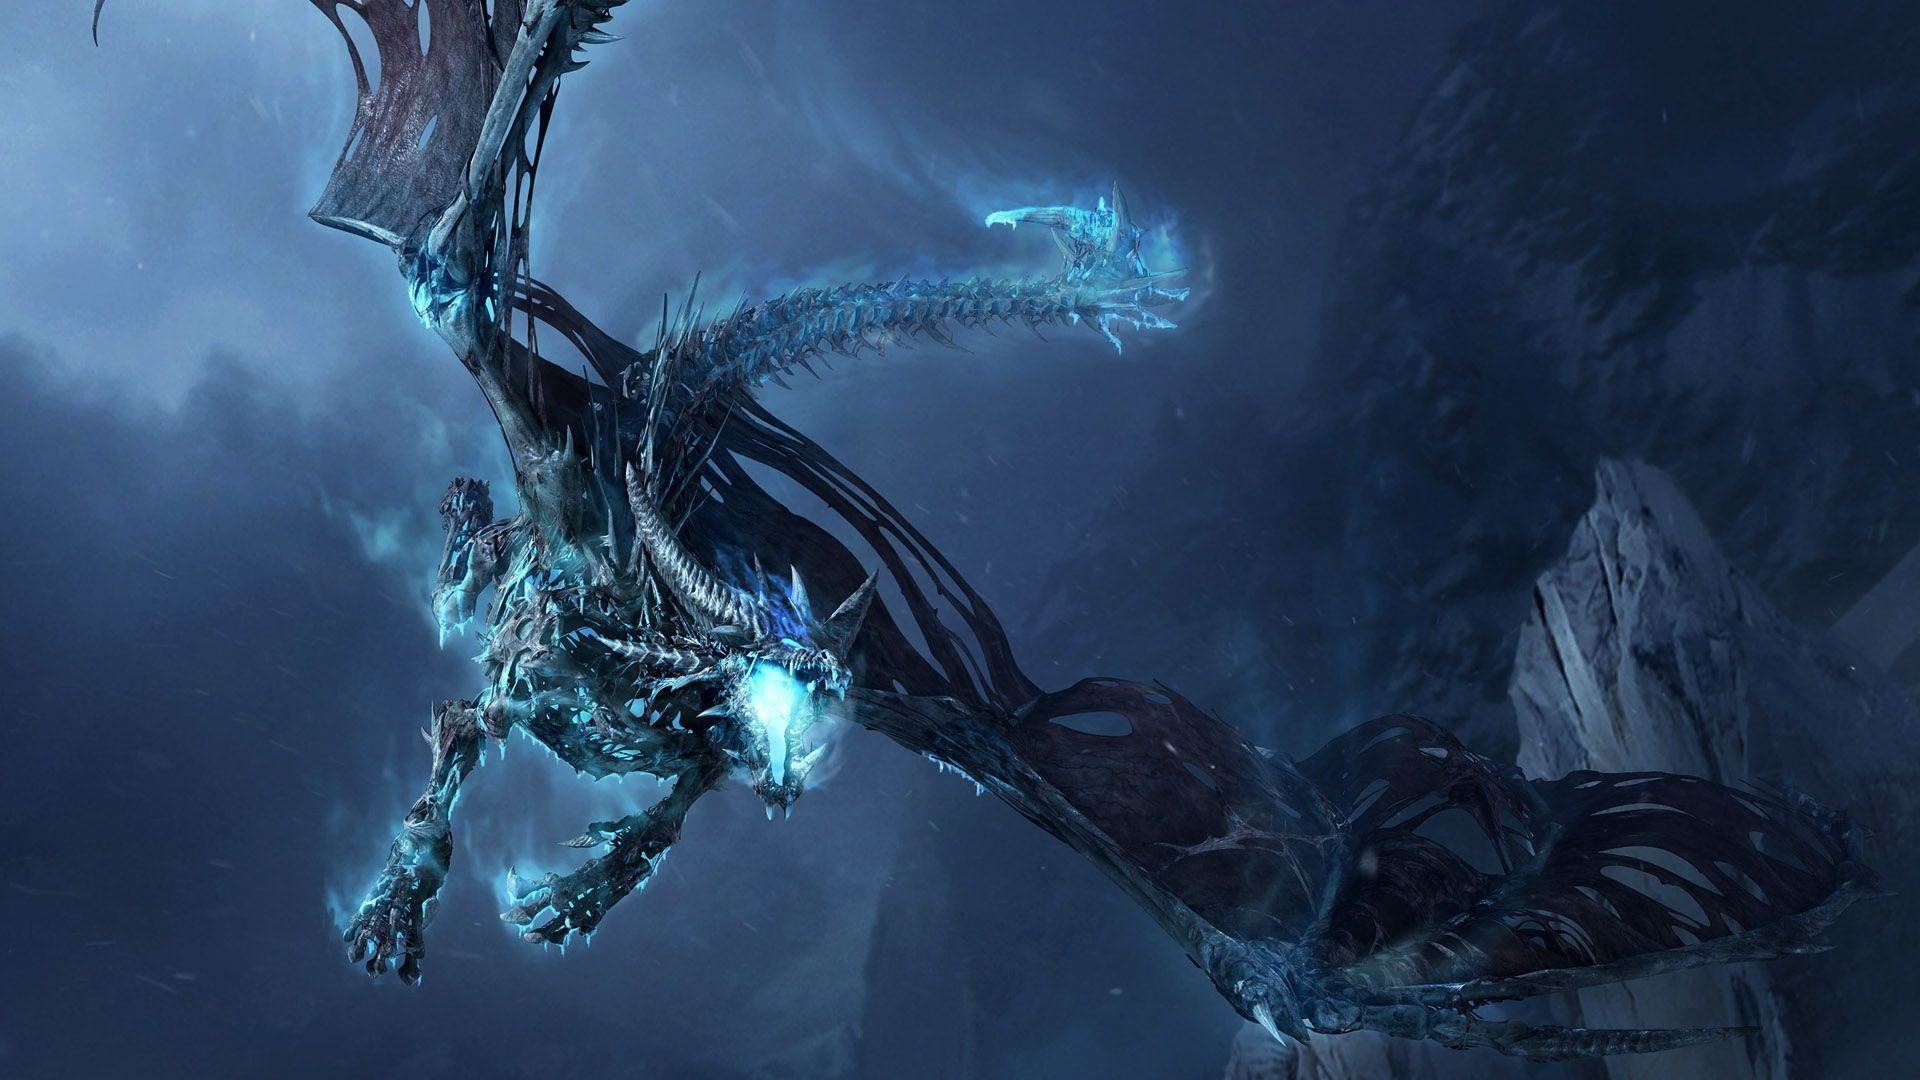
\includegraphics[width=0.7\linewidth]{img/WoW/crystaldragon.jpg}
	\end{center}

	Within the cavern of Crystalleous contains one of three magical rings created by Myrddin, a blue-gemmed ring. There are also other treasures that can be found within the cavern such as an ice rod, magic missile stave and other items from fallen foes who have traveled into the cavern. 
	
	\begin{center}
	
\includegraphics[width=0.7\linewidth]{img/maps/crystalleous.jpg}
	\end{center}
\end{commentbox}

\subsection{Xi'ra}

Xi'ra is a physical `god' created by Myrddin. Xi'ra was created as a being to perform specific duties only a deity could perform. Xi'ra was created to put a spiritual barrier around the Pluvian region and hide it from the sight of other ascended beings (gods). Xi'ra is hidden deep in the Pluvian forest and can only be found if the wearer has the three rings of the trinity dragons.





\section{Spati Aethereu Thalamun}

Spati Aethereu Thalamun (Space chamber, also sometimes referred to as just Aethereu) is the name of one of the Three Trinity Stone chambers. Specifically, This one is the space chamber. It was created by The Space Stone with remnants of the time and matter stones. Not much is known about this chamber. It is presumed to have been made when the Incantation to hide the Trinity stones was finished. The only way to reach Spati Aethereu Thalamun is to successfully travel through The Pluvian Forest. The reasons for the strange occurrences within The Pluvian Forest are believed to originate from this chamber by those who know the stories of it.

Aethereu is a trinity puzzle. There are many ways to navigate it but only one successful. Wrong navigations will lead to negative consequences. Each stone has an effect on the chamber which needs to be navigated simultaneously. If one, or two of three are done successfully but not the third, this is when a negative consequence happens.

First, the chamber consists of 13 triangular rooms. It can be represented by a hexagonal diagram.

\section{Auru Convallis}

This is the area to the East of Aurushire. This area is unexplored and all is known about it is that it is heavily dense with mountainous and forest terrain and the only known entrance path is through the southern shore which is blocked by a hostile Naga tribe.

\section{Endor (Moon)}

Endor is one of the two moons orbiting Orilla. Endor is where Camelot is located as a town/civilization established by Myrrdin. After Terra-forming Endor, a small group of individuals have been able to exist here to live by the law laid out by Myrddin. The moon itself is mainly dense forest and jungle region with some small mountains and a few open plains. There is limited wildlife other than what the villagers shepherd and breed.

\onecolumn
\chapter{Maps}
\section{Aurushire}
\begin{center}
	\includegraphics[width=\linewidth]{img/Aurushire.png}
	
	{\textbf{Aurushire:} To the south is the sea entrance. In the northwest is a secluded area where Baba Lives. To the northeast is a secluded area where Belmod lives. The North path leads to The Pluvian Forest and the West path leads to Rem Silva. The East side of the village is the location of Auru Convallis and the Naga camps are on the southeast side of the area leading into the eastern forest.}
\end{center}

\section{Rem Silva}
\begin{center}
	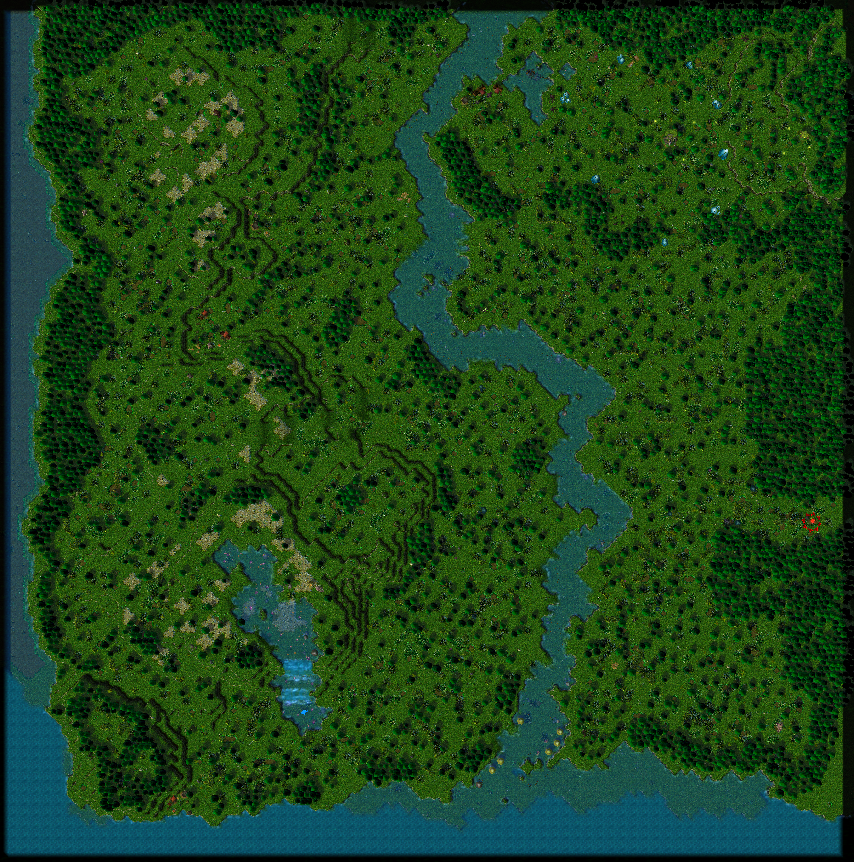
\includegraphics[width=\linewidth]{img/RemSilva.png}
	
	{\textbf{Rem Silva:} A forest to the west of Aurushire. To the north/Northeast is The Pluvian Forest but the forest is too dense to travel between the two.}
\end{center}

\section{Spati Aethereu Thalamun}
\begin{center}
	
\includegraphics[width=\linewidth]{img/Aethereu.png}	
	
	{\textbf{Aethereu:} The space chamber is composed of multi layered triangle rooms that can rotate about one another.}
\end{center}

\section{The Halls of No End}
\begin{center}
	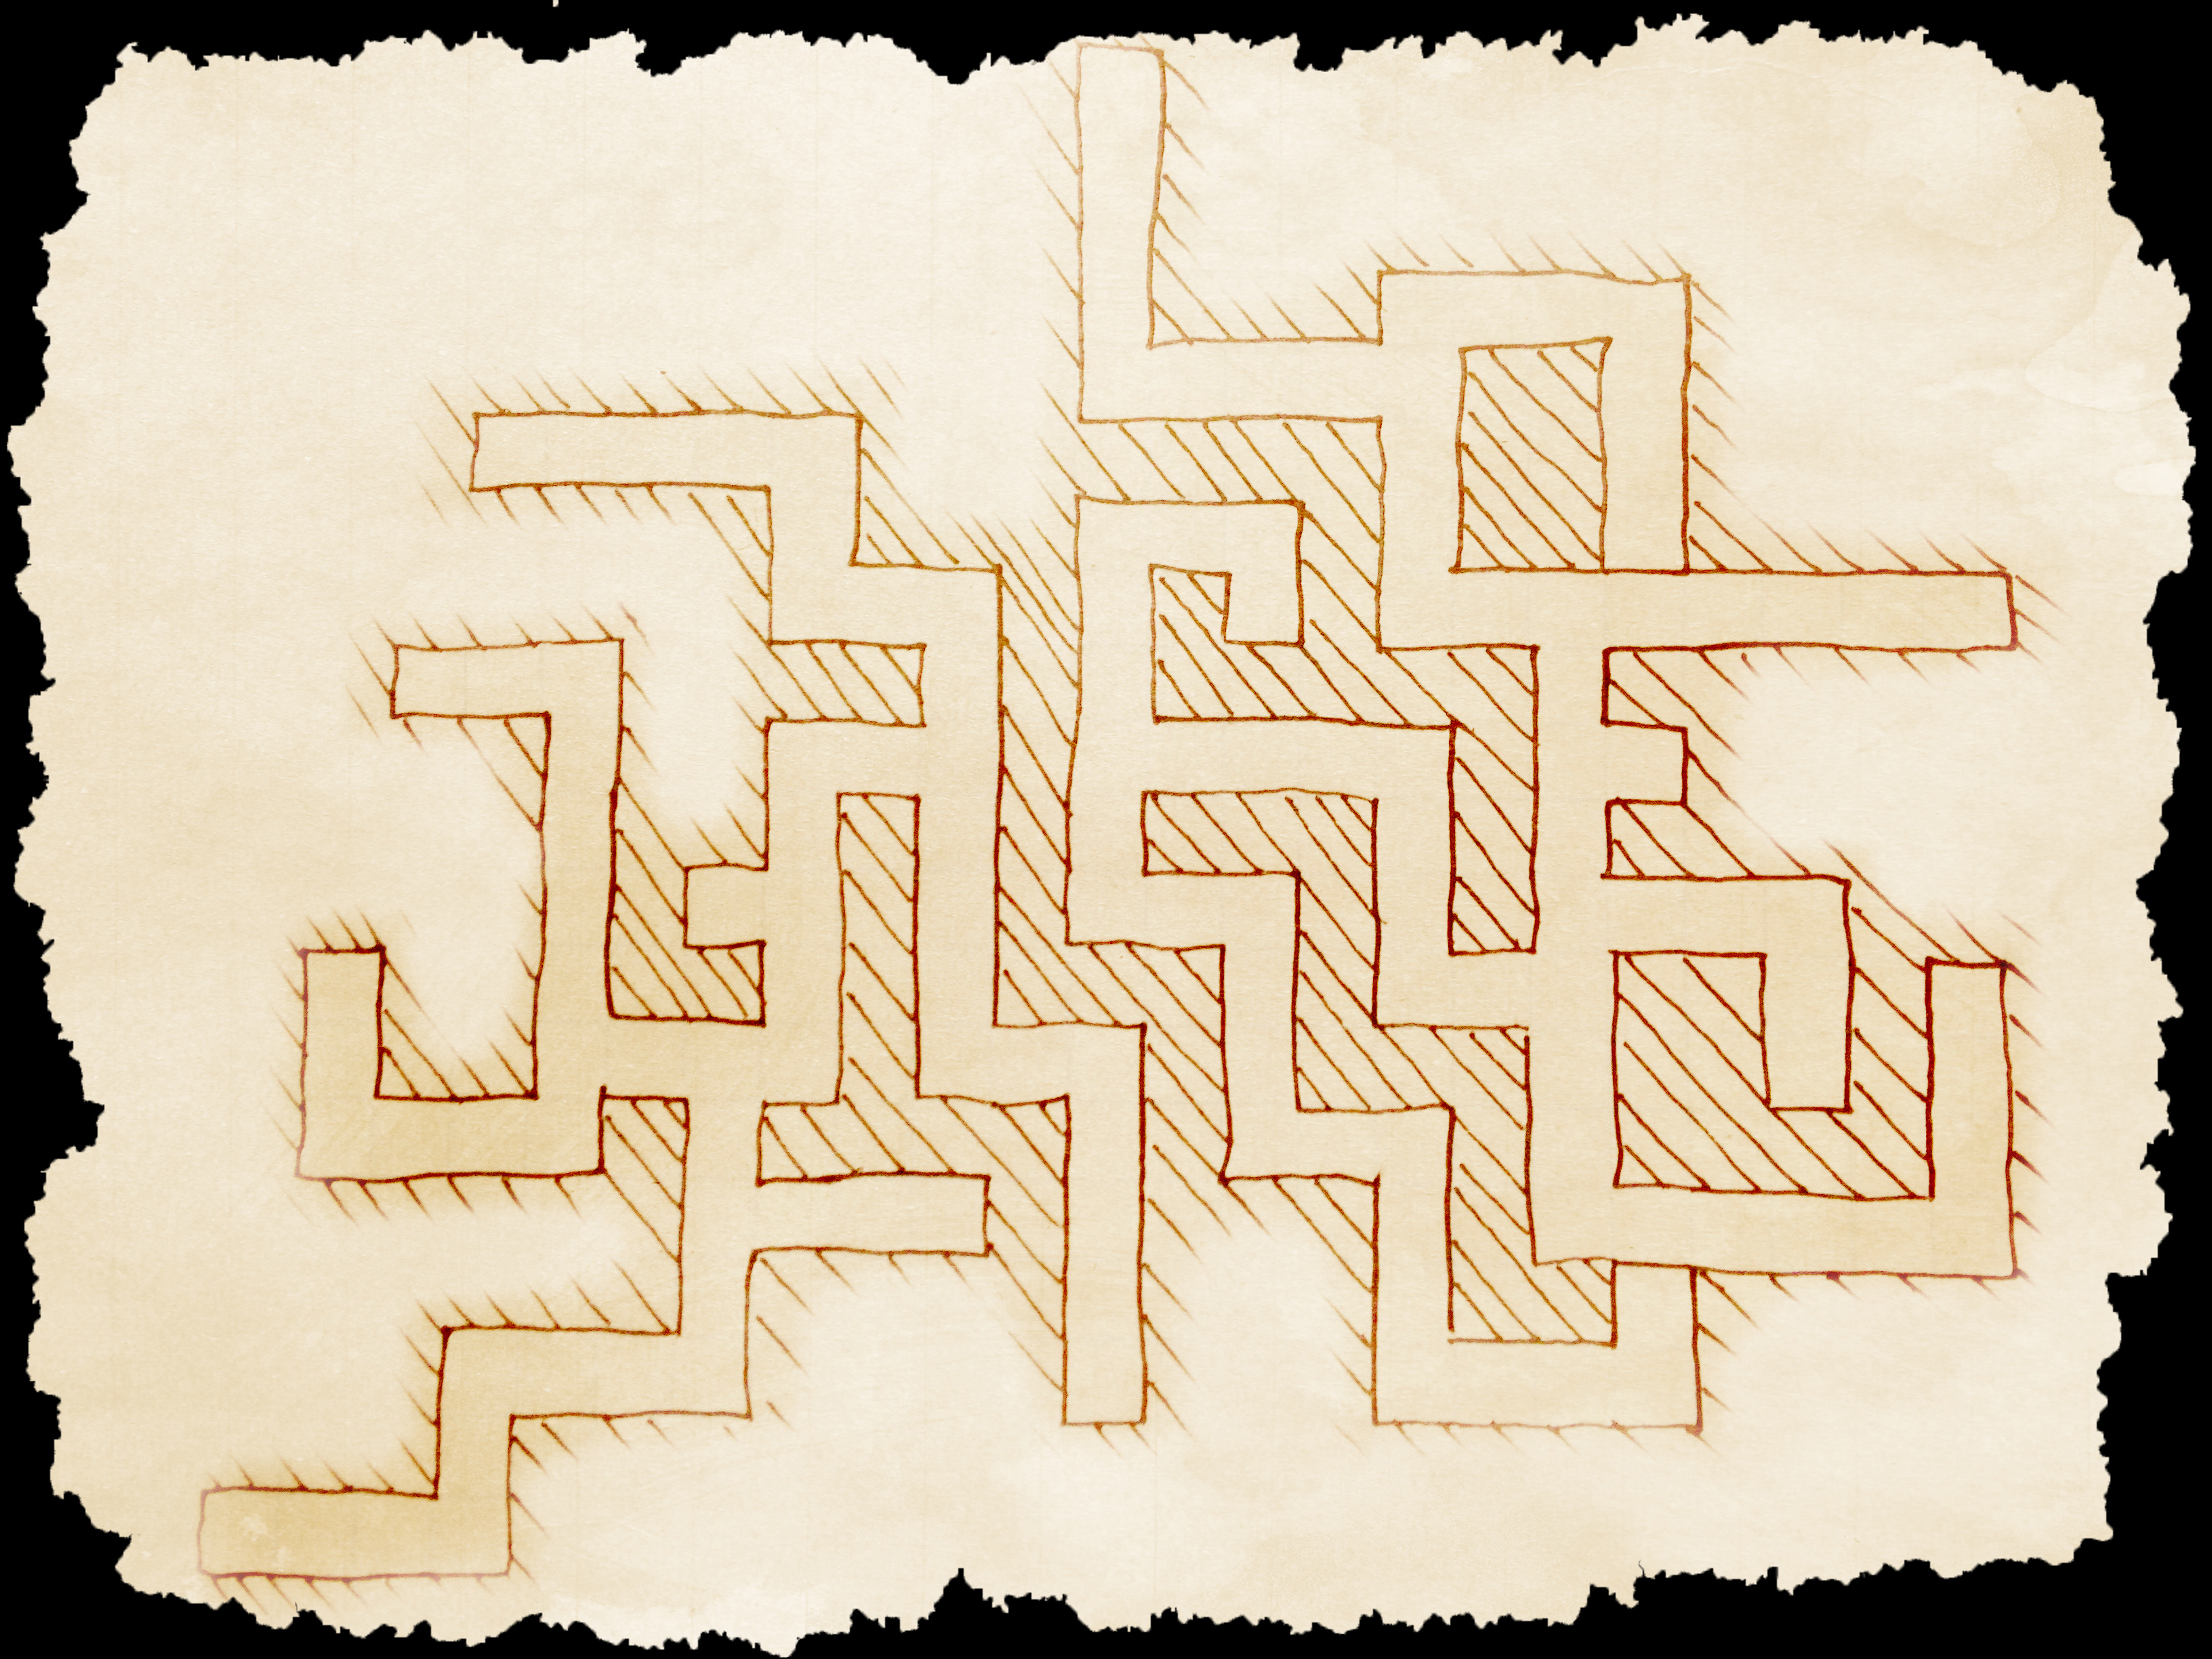
\includegraphics[width=\linewidth]{img/HONE.png} 
	
	{\textbf{Aethereu:} The Halls of no end is a puzzle area. There is one exit and it's the dead end which appears on the 2 long hallway to the left. Each hallway continues onto the hallway that is of the same length but opposite direction as it.}
\end{center}

% End document
\end{document}
